%% The first command in your LaTeX source must be the \documentclass command.
%%
%% Options:
%% twocolumn : Two column layout.
%% hf: enable header and footer.
\documentclass[
% twocolumn,
% hf,
]{ceurart}
\usepackage[utf8]{inputenc}
% \usepackage{cite}
\usepackage{amsmath,amssymb,amsfonts}
\usepackage{graphicx}
\usepackage{textcomp}
\usepackage{balance}
\usepackage{mathabx}
\usepackage{url}
\usepackage{subcaption}
\usepackage{pifont}
\usepackage{cleveref}
\usepackage{caption}
\usepackage{subcaption}
\usepackage{algorithm}
\usepackage[noend]{algpseudocode}
\Crefname{ALC@unique}{Line}{Lines}
\usepackage{float}
\usepackage{booktabs}
\usepackage{rotating}
\usepackage{enumitem}
\usepackage{ulem}
\usepackage{tablefootnote}
\newcommand{\specialcell}[2][c]{\begin{tabular}[#1]{@{}l@{}}#2\end{tabular}}
\newcommand{\cmark}{\ding{51}}%
\newcommand{\xmark}{\ding{55}}%
\newcommand{\eop}{\hfill $\Box$}  
\renewcommand{\sf}[1]{\textsf{\textup{#1}}}  
\renewcommand{\tt}[1]{\texttt{\textup{#1}}}
\definecolor{applegreen}{rgb}{0.55, 0.71, 0.0}
% \newcommand{\mf}[1]{{\color{blue}{#1}}}
\newcommand{\mf}[1]{#1}
\newcommand{\mfc}[2]{\mf{#1} {\color{red}{\textit{#2}}}}
\newcommand{\mg}[1]{{\color{red}{\textbf{#1}}}}
\newcommand{\eg}[1]{{\color{orange}{\textbf{#1}}}}
\algnewcommand\algorithmicforeach{\textbf{for each}}
\algdef{S}[FOR]{ForEach}[1]{\algorithmicforeach\ #1\ \algorithmicdo}
\algdef{SE}[DOWHILE]{Do}{doWhile}{\algorithmicdo}[1]{\algorithmicwhile\ #1}%
\newcommand{\algcolor}[2]{\hspace*{-\fboxsep}\colorbox{#1}{\parbox{\linewidth}{#2}}}
\newcommand{\algemph}[1]{\algcolor{lightgray}{#1}}

\newtheorem{theorem}{Theorem}
\newtheorem{example}{Example}
\newtheorem{definition}{Definition}
\newtheorem{formula}{Formula}
\newtheorem{proof}{Proof}

%%
%% end of the preamble, start of the body of the document source.
\begin{document}
\sloppy
\copyrightyear{2024}
\copyrightclause{Copyright for this paper by its authors. Use permitted under Creative Commons License Attribution 4.0 International (CC BY 4.0).}
\conference{SEBD 2024: 32nd Symposium on Advanced Database Systems, June 23-26, 2024, Villasimius, Sardinia, Italy}
\title{Colossal Trajectory Mining}
\subtitle{Semantic Co-movement Pattern Mining (Discussion Paper)}
\author[1]{Chiara Forresi}[orcid=0000-0001-5652-2455,email=chiara.forresi@unibo.it]
\address[1]{DISI --- University of Bologna, Cesena, Italy}
\author[1]{Matteo Francia}[orcid=0000-0002-0805-1051,email=m.francia@unibo.it]
\cormark[1]%\fnmark[1]
\author[1]{Enrico Gallinucci}[orcid=0000-0002-0931-4255,email=enrico.gallinucci@unibo.it]
\author[1]{Matteo Golfarelli}[orcid=0000-0002-0437-0725,email=matteo.golfarelli@unibo.it]
\author[1]{Manuele Pasini}[orcid=0009-0005-7023-6742,email=manuele.pasini@unibo.it]
%% Footnotes
% \cortext[1]{Corresponding author.}
% \fntext[1]{These authors contributed equally.}

%%
%% The abstract is a short summary of the work to be presented in the
%% article.
\begin{abstract}
Spatio-temporal mobility patterns are at the core of strategic applications such as urban planning and monitoring.
Depending on the strength of spatio-temporal constraints, different mobility patterns can be defined. 
While existing approaches work well in the extraction of groups of objects sharing fine-grained paths, the huge volume of large-scale data asks for coarse-grained solutions.
Colossal Trajectory Mining (CTM) efficiently extracts heterogeneous mobility patterns out of a multidimensional space that, along with space and time dimensions, can consider additional trajectory features (e.g., means of transport or activity) to characterize behavioral mobility patterns. 
The algorithm is natively designed in a distributed fashion, and the experimental evaluation shows its scalability with respect to the involved features and the cardinality of the trajectory dataset.
\end{abstract}

%%
%% Keywords. The author(s) should pick words that accurately describe
%% the work being presented. Separate the keywords with commas.
\begin{keywords}
Trajectory mining \sep Mobility patterns \sep Frequent itemset mining
\end{keywords}

%%
%% This command processes the author and affiliation and title
%% information and builds the first part of the formatted document.
\maketitle


\section{Introduction}\label{sec:intro}
The spreading of Internet of Things and mobile devices \citep{vitali2021crop} stimulated the rise of applications based on mobility patterns, such as urban mobility and traffic planning \citep{DBLP:journals/tits/KumarWRLKP18}, and moving objects (MOs) profiling and linking \citep{francia2020dart} where objects moving in similar locations can share interests or relationships.
Since different applications require identifying different mobility behaviors, researchers tailored a plethora of specific patterns.
However, the need for a \textit{unifying} analytic framework is well-understood and debated in the literature \citep{DBLP:journals/pvldb/DingCGJB18,DBLP:journals/jdwm/Kwakye20}.
% Ad-hoc implementations require ad-hoc extract-transform-load workflows, processing, and analysis; each of these steps entails expertise to maintain and operate each algorithm. Conversely, a holistic and unifying analysis solution is an important step towards applications that involve massive trajectory data \citep{DBLP:journals/pvldb/DingCGJB18} also enriched from heterogeneous sources.

Generally speaking, a \textit{mobility pattern} captures behaviors that frequently occur among MOs; each MO follows a trajectory that can be partially or completely shared with others.
Mobility patterns can be classified by the strength of the constraints on spatial and temporal proximity.
All patterns require spatial proximity to be satisfied for a sufficient length of the trajectories.
Conversely, temporal proximity is not always mandatory: a mobility pattern can be interesting even if the same path has been traveled at different times.
% \Cref{tab:proximitypattern} reports four widely studied patterns covered by our approach and shows application examples.
A co-location \citep{bao2021mining} is a group of objects located at the same points at any time (e.g., customers frequenting the same shops on different days).
Similarly, a flow \citep{DBLP:journals/tmc/HanLO15} is a co-location group where the path is contiguous (e.g., individuals moving through adjacent road segments).
A swarm \citep{DBLP:journals/pvldb/LiDHK10} is a group of objects moving within the same points at the same, possibly non-consecutive, time instants (e.g., individuals attending the same sport events each week).
Similarly, a convoy \citep{DBLP:journals/pvldb/JeungYZJS08} is a swarm group sharing (at least some) consecutive timestamps (e.g., individuals sharing a means of transport).

Most of the approaches in the literature focus on a specific pattern and a few unifying approaches have been introduced.
\cite{DBLP:journals/ijitdm/PhanPT16} and \cite{DBLP:journals/pvldb/FanZWT16} target small groups of objects sharing fine-grained paths, however, the huge volume of large-scale data (e.g., hundreds of thousands of trajectories spanning the entire USA) asks for coarse-grained solutions.
For instance, if our goal is to extract the groups of people flying across countries (e.g., USA has 50 states and 328 million inhabitants) or moving across city neighborhoods (e.g., Milan has 88 neighborhoods and 3 million inhabitants), meaningful groups are the ones in the order of hundreds/thousands of individuals. 
Indeed, extracting groups of 10 people given an average domestic flight of 150 people would return $\binom{150}{10} = 1.2 \cdot 10^{15}$ groups.

% Large-scale datasets demand a big-data solution, since (i) it could be impossible to load the entire dataset into main memory at once, and (ii) even if the dataset could fit into memory, millions of trajectories generate an exponential number of patterns.
%Such scenarios demand a big-data distributed solution, since (i) it could be impossible to load the entire dataset into main memory at once, and (ii) even if the dataset could fit into memory, millions of trajectories generate an exponential number of patterns.
% This is especially true for datasets where the number of trajectories, as well as their length in terms of points, is very large.
% Mobility patterns proposed in the literature look for (small) groups of MOs that, to some extent, share their trajectories.
% Due to the size of the search space and/or the centralized nature, such approaches fail when the goal is to capture huge groups of trajectories moving through limited spatial regions, 
% Furthermore, \cite{DBLP:journals/ijitdm/PhanPT16} and \cite{DBLP:journals/pvldb/FanZWT16} only address spatio-temporal patterns, preventing the possibility to characterize groups also in terms of additional features (e.g., means of transport, activity).

% \begin{table}[t]
% \centering
% \scriptsize
% \caption{Mobility patterns and examples of applications}

% \label{tab:proximitypattern}
% \begin{tabular}{ll}
% \toprule
% Pattern                                           & Application \\
% \midrule
% Co-location \citep{bao2021mining} & Frequent POI/route    \\
% Flow \citep{DBLP:journals/tmc/HanLO15}             & Historic traffic analysis\\
% Swarm \citep{DBLP:journals/pvldb/LiDHK10}          & Event \& Gathering\\ %Contact tracing\\
% Convoy \citep{DBLP:journals/pvldb/JeungYZJS08}         & Online traffic analysis\\%, convoy \citep{DBLP:conf/gis/GudmundssonKS04}
% % Platoon \citep{DBLP:journals/dke/LiBK15}         & Car sharing\\
% \bottomrule
% \end{tabular}%
% \end{table}

In this paper, we describe Colossal Trajectory Mining (CTM), previously introduced in \cite{DBLP:journals/eswa/FranciaGG24}, an approach that generalizes many of the previous approaches while overcoming their limitations and integration effort.
CTM 
(i) is a unifying framework for the extraction of heterogeneous mobility patterns; 
(ii) is suitable for applications working on datasets with a huge number of (long) trajectories traveling across limited spatial regions (i.e., \#trajectories $\gg$ \#regions);
% \item it generalizes the mobility patterns reported in \Cref{tab:proximitypattern} through generic spatio-temporal constraints;
(iii) characterizes MOs through a tessellation including spatial and temporal features as well as additional features that enable the comprehension of semantic mobility behaviors \citep{DBLP:journals/tist/Yan0PSA13} (e.g., characterizing mobility behaviors by means of transport or activity);
% \footnote{Note that the tessellation is given as input and the tuning of its granularity is out of the scope of the paper (see \Cref{sec:related}); we introduce an algorithm to mine co-movement patterns out of any (possibly semantic) tessellation.};
and (iv) does not require similarity computation between trajectories, preventing the design of burdensome metrics.
    % \item it is implemented following the big-data paradigm, enabling high scalability in terms of both input trajectories and extracted patterns.
% \end{itemize}
% We emphasize that the terms ``\textit{colossal} (trajectory) mining'' and ``\textit{big} data'' have different meanings. Colossal \citep{DBLP:conf/kdd/PanCTYZ03} is an application of mining techniques to datasets having the number of dimensions (columns) sensibly higher than the number of instances (rows)\footnote{This happens, for example, in biological datasets such as gene expression datasets that may contain $10^5$ columns but only $10^3$ rows \citep{DBLP:conf/kdd/PanCTYZ03}.}; colossal mining can require big data techniques, where big data refers to datasets (that produce results) that are too large to be dealt with by centralized data-processing applications.
%.Such datasets pose a great challenge for existing (closed) frequent pattern discovery algorithms, since they have an exponential dependence on the average row length

The remainder of the paper is organized as follows.
In \Cref{sec:related}, we position and compare our approach with respect to the related literature.
In \Cref{sec:Overview}, we describe CTM.
% Then, we formalize the theoretical foundations of our approach in \Cref{sec:modeling}, we provide its implementation in \Cref{sec:mining}, and we discuss its complexity in \Cref{sec:complexity}.
% Then, we formalize the theoretical foundations of our approach in \Cref{sec:modeling}, and we provide its implementation in \Cref{sec:mining}.
In \Cref{sec:test}, we assess the effectiveness and efficiency of CTM by leveraging both real-world and synthetic case studies. 
Finally, we summarize our approach and future research directions in \Cref{sec:conclusion}.


\section{Related work}\label{sec:related}

% CTM intersects frequent itemset mining and clustering. 
\textbf{Frequent Itemset Mining} uncovers co-occurrences among the items in a transaction dataset \citep{DBLP:conf/vldb/AgrawalS94}. 
FIM has been also applied to trajectory data to find routes \citep{DBLP:conf/ideal/QiuP16,DBLP:journals/access/FuTXZ17} or regions \citep{zheng2018spatial} frequently trafficked by MOs.
This is an \textit{orthogonal} problem to extracting groups of objects moving together.
%(e.g., a trajectory might support multiple routes and a route might be supported by dissimilar trajectories).

Colossal itemset mining is a branch of FIM that computes FI in highly-dimensional datasets; for instance, a dataset with 30 transactions/rows/instances each with 10$^7$ items/columns \citep{DBLP:journals/bdr/ApilettiBCGPM17}.
% With respect to CTM, 
% Previous colossal itemset mining algorithms, such as 
Carpenter \citep{DBLP:conf/kdd/PanCTYZ03} generates frequent closed itemsets in a depth-first centralized fashion.
% In a centralized architecture, Carpenter exploits an in-memory accumulator in which all patterns are stored; this cannot scale to data that do not fit into main memory: even if the transaction dataset can fit into main memory in a single machine, the exponential number of co-movement patterns might not.
In \cite{DBLP:journals/bdr/ApilettiBCGPM17}, the authros distribute the branches of the depth-first exploration over distributed executors. 
However, (i) this results in highly unbalanced partitions,
and (ii) a centralization mechanism must be iteratively applied to discard redundant branches (i.e., patterns are redundantly generated).
% since in a distributed scenario there is no shared memory, 
% Additionally, since memory is not shared by executors, they cannot share the accumulator; without a shared data structure, patterns are redundantly generated. 
% Accumulating all the patterns into a single executor is troublesome, since 
% and (iii) shuffling all the patterns is a data-intensive operation.
% that burdens a single executor. Also, even if possible, the number of co-movement patterns is limited by the resources of a single executor (a single point of failure).
While other algorithms for colossal itemset mining have been recently proposed \citep{DBLP:conf/kdd/PanCTYZ03,DBLP:journals/kbs/ZakiZ18,DBLP:journals/isci/VanahalliP19}, \textit{none} address the extraction of constrained co-movement patterns.
%nor introduce pruning strategies for spatio-temporal data. 

% \subsection{Clustering}
\textbf{Clustering}
% Movement pattern mining and trajectory clustering are similar topics. 
% Indeed, 
groups trajectories such that intra-group similarity is maximized and inter-group similarity is minimized. 
% are extracted through trajectory clustering algorithms. 
% While many clustering algorithms have been proposed, only a few group trajectories under spatio-temporal constraints (e.g., continuous time, minimum time, cohesion) required by movement patterns.
% \mg{stringere a manetta la parte sul clustering e spostare il resto in related}
% Trajectory 
% Clustering techniques are characterized by the \textit{rationale} and the \textit{similarity metric}.
%that are leveraged to produce groups (i.e., sets of trajectories) that maximize intra-cluster similarity and maximize inter-cluster diversity.
% As to the rationale, \textit{flow-based} clustering can group trajectories with very limited overlapping \citep{DBLP:conf/icdcs/HanLO12,DBLP:journals/tmc/HanLO15}; for instance, after a map-matching phase \citep{DBLP:conf/mipro/FranciaGV19}, cars traveling different segments of the same road determine a flow along the road.
% \textit{Partitioning} clustering groups whole trajectories \citep{DBLP:journals/tkde/HanLO17,DBLP:journals/tits/KumarWRLKP18,DBLP:journals/pvldb/WangBCSQ19} and does not preserve inter-cluster patterns (e.g., common sub-trajectories).
% Indeed, while a trajectory is grouped with similar ones, still it can share interesting paths with trajectories from other clusters.
% \textit{Overlapping} clustering \citep{DBLP:conf/sigmod/LeeHW07,tampakis2019scalable,ailin2019movement} splits trajectories into sub-trajectories and groups them.
% However, even if at a smaller scale, this leads to the loss of so-called rare patterns, namely meaningful spatial events occurring with a low frequency \citep{DBLP:journals/tkdd/KohR16}.
% As a consequence, all these rationales are limited since they do not preserve groups sharing a few points (which can be strategic).
% As to the similarity definition, the higher the expressiveness, the higher the computational complexity.
% The Euclidean distance \citep{van1995some} has linear complexity in trajectory length but requires equally-long trajectories and does not detect time shifts. 
% DTW \citep{DBLP:conf/kdd/RakthanmanonCMBWZZK12} overcomes these limitations and is robust to missing points but at the cost of quadratic complexity.
% Further distance functions are Hausdorff \citep{DBLP:journals/tip/SimKP99} (the greatest of all the distances from a point in one trajectory to the closest point in the other trajectory), LCSS (\cite{DBLP:conf/icde/VlachosGK02}; similarity is expressed in terms of the longest common subsequence of two trajectories), Frechet (\cite{DBLP:conf/pods/AgarwalFMNPT18}; the smallest of the maximum pairwise distances), and road based (\cite{DBLP:conf/mdm/SilvaLMZC20}; the minimum number of network paths between two trajectories in a certain time window).
% Different distance functions produce different clusterings; \cite{DBLP:conf/icde/VlachosGK02} compare LCSS, Euclidean, and DTW.
% However, these \textit{spatio-temporal} distances cannot be directly adopted in our approach for the following reasons:
% \begin{itemize}
% \item they do not consider further geometric (e.g., speed or direction) or semantic (e.g., point types or means of transport) features;
% \item they cannot be applied at different aggregation levels (e.g., neighborhoods and cities);
% \item they cannot be applied to all co-movement patterns (e.g., LCSS, which returns as similar trajectories sharing a contiguous path, is not suitable for the co-location pattern where path adjacency is not required).
% \end{itemize}
Since ``classic'' clustering algorithms \textit{do not} enforce a definition of co-movement patterns (e.g., cardinality, time span, cohesion, spatial and/or temporal contiguity), flock \citep{DBLP:conf/gis/GudmundssonK06}, convoy \citep{DBLP:journals/pvldb/JeungYZJS08}, and swarm \citep{DBLP:conf/ssdbm/AungT10} patterns have been formalized.
As swarm \citep{DBLP:conf/ssdbm/AungT10} groups objects moving in spatial proximity for a given amount of possibly-non-contiguous time,
classical clustering algorithms can be referred to as swarms if no minimal duration is enforced.
% Finally, all these approaches produce clusters of raw trajectories \textit{without} the possibility to cluster trajectories under custom and semantic dimensions (e.g., regions of interest, MO type, and activity).

% \subsection{Distinguishing features of CTM}
% \textbf{Distinguishing features of CTM.}
% Since MOs outnumber the regions of interest, CTM is a novel perspective in the analysis of mobility patterns.
% The research on co-movement patterns is active;
% recent relevant papers work toward improving the mining efficiency through spatial hierarchical constraints \citep{helmi2020multiscale} or by providing pattern-specific strategies; for instance filtering convoys in either a centralized \citep{DBLP:conf/ssdbm/AungT10,DBLP:journals/pvldb/OrakzaiCP19,DBLP:conf/cikm/Liu0LLYW21} or distributed \citep{DBLP:journals/geoinformatica/OrakzaiPC21,tritsarolis2022predicting} fashion.
% %) and co-location (either centralized \cite{lv2019discovering,tran2021spatial} or distributed \cite{fonseca2022multi}).
% Our goal is providing a unifying framework for pattern analysis.
% The need for a unifying framework is well-understood and debated in literature \citep{DBLP:journals/pvldb/DingCGJB18,DBLP:journals/jdwm/Kwakye20}.
% \cite{DBLP:journals/ijitdm/PhanPT16} and \cite{DBLP:journals/pvldb/FanZWT16} are close contributions to CTM and both extract spatio-temporal mobility patterns by discretizing time in bins, clustering MOs in every bin, and merging clusters across bins.
\Cref{tab:related} summarizes the comparison with existing approaches.
% ; the strengths of CTM are the following.
% \begin{enumerate}
%     \item Transparently and homogeneously supporting semantic features to characterize behavioral mobility patterns (e.g., neighborhood and municipalities, means of transport, holiday or work day; \Cref{fig:milnil,fig:milmun}).
%     Geometric-only (e.g., spatio-temporal) tessellations are supported but they are only one of the possible tessellation types.
%     This makes CTM extensible in the characterization of behavioral mobility patterns. 
%     \item Extracting spatial, spatio-temporal, and semantic patterns ---whereas \cite{DBLP:journals/ijitdm/PhanPT16,DBLP:journals/pvldb/FanZWT16} require an \textit{absolute} temporal dimension--- by applying constraint and pruning strategies that allow to return several pattern types as well as to reduce the algorithmic search space.
%     \item Providing a native distributed solution to the problem that can scale up to real-world datasets and a lossless compression of the output patterns by leveraging frequent closed itemsets.
% \end{enumerate}
% While CTM could be associated with grid-based clustering, automatically finding the best grid for a specific dataset/problem/co-movement pattern is out of the scope of the paper.
% To ease the computation of similarity, grid-based clustering uses a grid to build the clusters out of adjacent densely-populated cells.
% Setting the resolution grid is difficult \citep{parsons2004evaluating,DBLP:journals/tkde/JinHZXFOZ22}, especially in multi-dimensional datasets with heterogeneous densities across dimensions.
% In this case, even adaptive grids \citep{DBLP:conf/adma/LuSXL05}
% are not a solution since they raise the following dataset- and problem-specific issues.
% \begin{itemize}
%     \item \textit{Dataset-specific}: computing the ``best'' tessellation requires to define what are the ``best'' co-movement patterns.
%     Internal metrics measure how distinguishable clusters are without the need for external knowledge.
%     For instance, the silhouette index measures whether crisp partitioning clusters are compact and well-separated \citep{zhu2010clustering}.
%     However, co-movement patterns can be overlapping since trajectories can contribute to multiple groups of MOs.
%     External metrics require labels to find the ``best'' co-movement patterns out of the given dataset/tessellation (e.g., the ``purity'' of clusters through entropy); this type of supervised evaluation is usually leveraged to compare different grid-based algorithms \citep{parsons2004evaluating}.
%     Besides the metrics, defining the ``best'' co-movement patterns also depends on the dataset heterogeneity; e.g., taxis in \citep{DBLP:conf/gis/YuanZZXXSH10} produce homogeneous and precise trajectories, while Movebank \citep{DBLP:journals/envsoft/KranstauberCWFTWK11} collects data from thousands of studies.
%     \item \textit{Problem-specific}: co-movement patterns depend on (i) the goal of the analysis (e.g., monitoring co-movement patterns at single user levels at the scale of meters, or aggregated network data
%     %\cite{zhang2020exploring}
%     at the scale of kilometers); and (ii) the type of moving objects (e.g., to retrieve a convoy of 5 people moving in the same car a cell of 6 square meters could be enough, but this is not true to detect convoys of cars or trucks spanning hundreds of meters ---for instance in a highway).
% \end{itemize}

\begin{table}[t]
\centering
\scriptsize
\caption{Excerpt of the comparison with existing co-movement patterns approaches}% by supported features and pattern types and distributed implementation}
\label{tab:related}
\begin{tabular}{lcccccl}
\toprule
Features & Co-location & Flow & Convoy & Swarm & Distributed & Contributions \\
\midrule
Any & \cmark & \cmark & \cmark & \cmark & \cmark & CTM \\
Space & - & \cmark & - & - & - & \cite{DBLP:conf/mdm/SilvaLMZC20}, \cite{yang2021scpm}, \cite{tritsarolis2021online} \\
% Space & \cmark & - & - & - & - & \cite{lv2019discovering}\\%\\, \cite{tran2021spatial} \\
Space & \cmark & - & - & - & \cmark & \cite{fonseca2022multi} \\
Space, Time & - & - & - & \cmark & - & \cite{DBLP:conf/sigmod/LeeHW07}, \cite{DBLP:journals/pvldb/LiDHK10}\\%, \cite{DBLP:journals/tkde/HanLO17}, \cite{ailin2019movement}, \cite{li2023relaxed} \\
Space, Time & - & - & - & \cmark & \cmark & \cite{DBLP:conf/icnc/HuKLZ15}, \cite{tampakis2019scalable} \\
Space, Time & - & - & \cmark & - & - & \cite{DBLP:conf/ssdbm/AungT10}, \cite{DBLP:journals/pvldb/OrakzaiCP19}, \cite{DBLP:conf/cikm/Liu0LLYW21} \\
Space, Time & - & - & \cmark & - & \cmark & \cite{DBLP:journals/geoinformatica/OrakzaiPC21}, \cite{tritsarolis2022predicting} \\
% Space, Time & - & - & \cmark & \cmark & - & \cite{DBLP:journals/dke/LiBK15}, \cite{DBLP:journals/ijitdm/PhanPT16}, \cite{helmi2020multiscale} \\
Space, Time & - & - & \cmark & \cmark & \cmark & \cite{DBLP:journals/pvldb/FanZWT16} \\
Space, Time & - & \cmark & - & - & - & \cite{DBLP:journals/tmc/HanLO15}, \cite{DBLP:journals/tits/KumarWRLKP18}, \cite{DBLP:journals/pvldb/WangBCSQ19} \\
\bottomrule
\end{tabular}
\end{table}

\section{Mining semantic co-movement patterns}
\label{sec:Overview}

% Modeling mobility pattern mining as a \textit{colossal} frequent itemset problem is a novel research direction. 
% The goal of Frequent Itemset Mining \citep{DBLP:conf/vldb/AgrawalS94}, historically used for market-basket analysis, is to extract \textit{items} (e.g., products) that often appear together in a dataset of \textit{transactions} (e.g., receipts of product sales). 
% Similar to the sales problem, FIM retrieves sets of trajectories (i.e., items) moving together in the same places (i.e., transactions). 
% Colossal refers to the scenario in which the number of traveled places is sensibly lower than the number of trajectories \citep{DBLP:conf/kdd/PanCTYZ03}.

% \begin{figure}[t]
%     \begin{subfigure}[t]{.49\columnwidth}
%         \centering
%         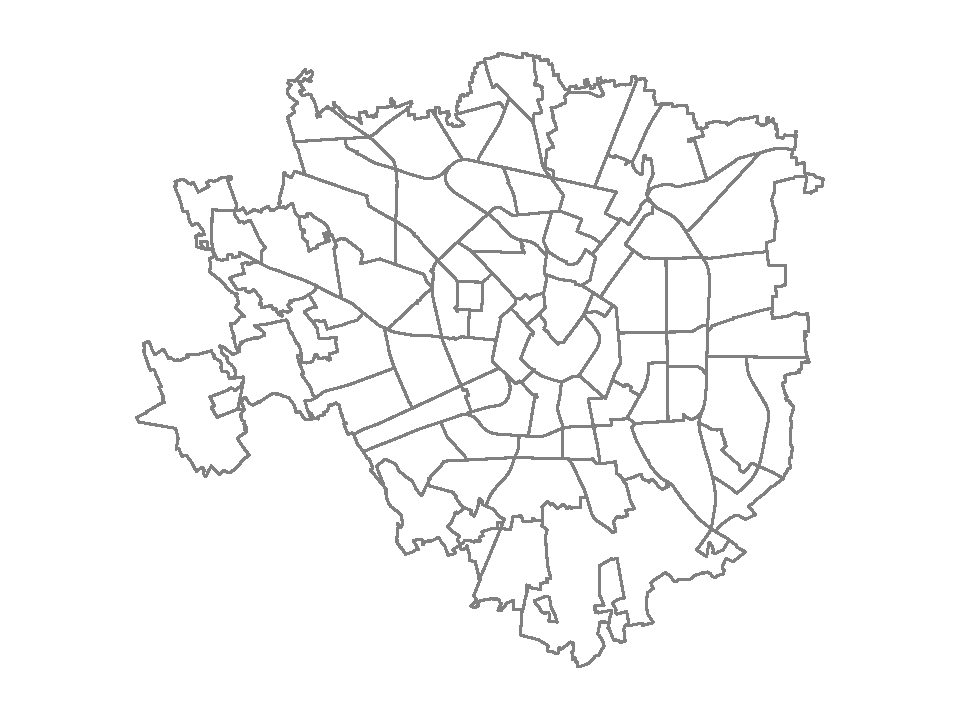
\includegraphics[width=.8\textwidth]{milan-nil.pdf} %us-counties-cut
%         \caption{Neighborhoods}
%         \label{fig:milnil}
%     \end{subfigure}~
%     \begin{subfigure}[t]{.49\columnwidth}
%         \centering
%         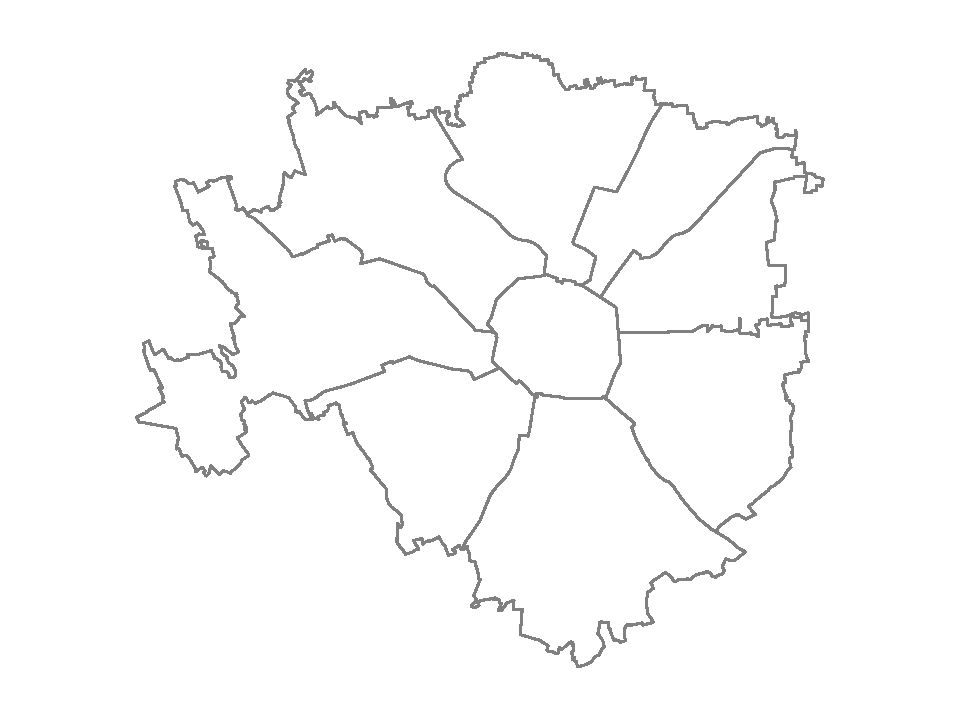
\includegraphics[width=.8\textwidth]{milan-munic.pdf} % us-states-cut
%         \caption{Municipalities}
%         \label{fig:milmun}
%     \end{subfigure}
%     \caption{Administrative spatial tessellations of Milan.}
%     \label{fig:multilevtess}
% \end{figure}

\begin{figure}[t]
    \centering
    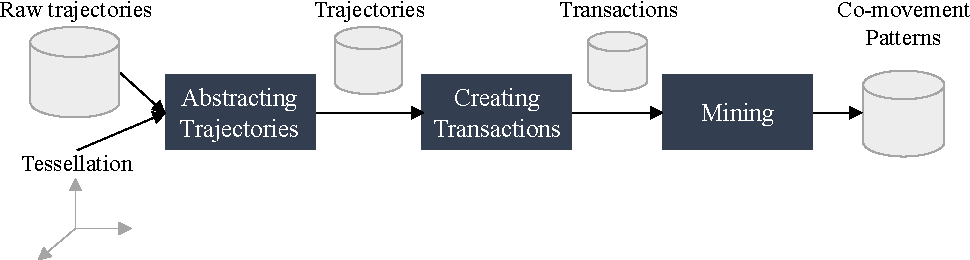
\includegraphics[scale=.7]{overview.pdf}
    \caption{Overview of CTM.}
    \label{fig:overview}
\end{figure}

Our approach is based on the following steps (\Cref{fig:overview}).

\subsection{Abstracting trajectories}

We consider a dataset of raw trajectories, where each trajectory point is labeled with a set of features.
Mandatory features are those needed to define spatial or spatio-temporal locations (e.g., latitude, longitude, and timestamp), but other semantic features might be available.% (e.g., speed, day of the week, and neighborhood).

\begin{definition}[Raw trajectory and feature] 
A \textit{raw trajectory} $P$ is a sequence of points $(p_1, \ldots, p_{|P|})$ generated by a MO. 
The \textit{feature space} is a set of features $F=\{f_1,\ldots,f_{|F|}\}$ that is collected for each point.
% ; it represents a multidimensional space where each dimension corresponds to a feature.
\end{definition}

Raw trajectories are mapped to a multidimensional tessellation, a composition of multidimensional tiles (from now on, simply \textit{tiles}) of \textit{any} shape --- with no overlaps and no gaps --- that cover a multidimensional space; the tessellation \textit{is not} necessarily a regular grid.
% the covering of muldimensional space using one or more tiles (shapes) with no overlaps and no gaps.
Each dimension of the tessellation corresponds to a feature describing the raw trajectory points: common features are space and time, but additional features can be added to specialize each trajectory point (e.g., whether an individual is moving by car or by bicycle).
This allows grouping trajectories on semantic and behavioral concepts (e.g., to capture groups of individuals moving across city neighborhoods with different means of transport).

\begin{definition}[Tessellation] 
% Given a dataset of raw trajectories associated with the features $F$, 
We call \textit{tessellation} a multidimensional partitioning $S = \{s_1, \ldots, s_m\}$ of the feature space $F$.
Each \textit{tile} of the tessellation is identified by an $id$ and is characterized by an interval/set of values for each continuous/nominal feature in $F$.
For each feature $f$, the function $dist_f(s_i, s_j)$ computes the distance between two tiles on the tessellation.
Two tiles $s_i$, $s_j$ $\in S$ are  \textit{adjacent} ($s_i \cong_{f} s_j$) if $\forall s_z \in S$ it is $dist_f(s_i,s_j)\leq dist_f(s_i,s_z) + dist_f(s_z,s_j)$.
\end{definition}

% Note that $dist_f()$ is a distance between tiles used to characterize different mobility patterns.
% Since in a colossal problem the number of tiles is  order of magnitude lower than the number of trajectories and trajectory points, computing distances between tiles entails a computational complexity that is by far lower than working on raw trajectories.
In our implementation, the distance function is
\begin{equation}
dist_f(s_i,s_j) =
\bigg \{
\begin{array}{ll}
f \textup{ is ordinal}  & geod(s_i,s_j) \\
f \textup{ is nominal} \wedge s_i = s_j & 0 \\
f \textup{ is nominal} \wedge s_i \neq s_j & \infty \\
\end{array}
\end{equation}
%
where $geod(s_i,s_j)$ is the geodesic distance \citep{bouttier2003geodesic} computed on the tessellation, which is the number of tiles along the shortest path of neighboring tiles connecting $s_i$ and $s_j$.

\begin{definition}[Tile connection]\label{def:adj} 
Two tiles $s_i,s_j$ in the tessellation $S$ are  \textit{connected} ($s_i \leftrightarrow_{f} s_j$) if there exists a path of adjacent tiles in $S$ connecting them in $f$.
\end{definition}
% Although in principle any distance metric can be leveraged (e.g., Haversine or Euclidean), using the geodesic distance simplifies the formalization of co-movement patterns.
% As to nominal features (e.g., monitoring urban traffic on weather conditions such as rainy/sunny) that do not allow ordering, the distance function allows the selection of homogeneous tiles, and in turn, searches for co-movement patterns characterized by the same nominal values.
%$s_i,s_j$ are  \textit{adjacent} ($s_i \cong_{f} s_j$) if $geod(s_i,s_j) \le 1$.

A trajectory is an abstraction of a raw trajectory at the grain defined by the tessellation.

\begin{definition}[Trajectory] 
\label{def:tes}
Given a raw trajectory $P$ and a tessellation $S$, we define the \textit{trajectory} $T$ corresponding to $P$ in $S$ as the sequence of tiles $(s_{1}, \ldots, s_{|T|})$ such that a tile $s$ is added to $T$ if at least a point $p \in P$ is in $s$.
% ; formally, $p\in s$ if $p_f \in s_f, \forall f \in F$.
A point $p$ \textit{is in} the tile $s$ if, for each feature in $F$, the values of the feature for $s$ contain the corresponding feature value characterizing $p$.
\end{definition}

Noticeably, the tessellation:
% The grain of each tile determines the scale and precision of the tessellation.
% \begin{itemize}
% \item 
(i) defines the level of the analysis (CTM transparently allows the extraction of patterns at neighborhood/city/country scales) 
%(\Cref{fig:multilevtess}) 
and (ii) compresses trajectories since a trajectory \textit{moves through} a tile if at least one of its points belongs to the tile (a single tile instance is added to $T$ if consecutive points fall in that tile, thus $|P| \geq |T|$).
%(i.e., there is no need to store consecutive points from the same tile more than once). This makes the computational complexity more related to the scale of tessellation rather than to the trajectories length. For this reason, CTM is particularly suited for applications working on a huge number of, potentially long, trajectories and a coarse tessellation.
% \item The tessellation implicitly defines similarity: the more tiles two trajectories share, the higher their similarity.
% \end{itemize}
% This determines a first data compression: .



% \begin{example}[Tessellation, tile, and trajectory]\label{ex:trajabst}
% With reference to \Cref{fig:patterns2}, the grid is a tessellation involving the spatial feature $f^{sp}$ which characterizes 16 tiles (i.e., cells from $A1$ to $D4$); $dist_{f^{sp}}(A1,A2) = 1$ and $dist_{f^{sp}}(A1,A3) = 2$; the point 
% % p $\in B2$
% $p$ is in the tile $B2$ and the trajectory $T_r=(A1,B1,B2,B3,D3)$ corresponds to the red raw trajectory within the tessellation.
% \end{example}


\subsection{Creating transactions}
% To each tile corresponds a transaction including the trajectories (i.e., items) moving through it.

To formalize CTM as a colossal itemset mining problem, we introduce \textit{transactions} and \textit{items}.
% Each transaction corresponds to a tile and includes the items/trajectories moving through that tile.

\begin{definition}[Item, itemset, and transaction] Given a trajectory dataset $\mathcal{T}$ and a tessellation $S$, each trajectory represents an \textit{item}, and a set $I$ of trajectories is an \textit{itemset}.
We define the \textit{transaction} for a tile $s \in S$ as the itemset containing all the trajectories having at least a point in $s$.
$\mathcal{Q}$, the set of all transactions, is a transaction dataset.
\end{definition}

As transactions are \textit{sets} of items, the data is further compressed: if a tile is traversed more than once by a trajectory, the transaction (tile) will contain the item (trajectory) only once.

Since we are looking for trajectories sharing feature values, we need to identify the itemsets contained in a large number of transactions. 
This property is captured by the support function.

\begin{definition}[Support]
Given a transaction dataset $\mathcal{Q}$, the \textit{support} $sup(I)\subseteq\mathcal{Q}$ of an itemset $I$ is the set of transactions containing $I$.
\end{definition}

% \begin{example}[Itemset, transaction, and support]
% With reference to \Cref{fig:patterns2}, $Q_{A1}=\{T_b,T_g,T_r\}$ is the transaction corresponding to the tile $A1$, $I=\{T_g,T_r\}$ is an itemset, and $sup(I) = \{Q_{A1}, Q_{B1}, Q_{B2}, Q_{B3}\}$.
% \end{example}

\begin{definition}[Frequent and closed itemsets]\label{def:fci}
An itemset is $I$ \textit{frequent} (FI) if $|sup(I)|\geq mSup$, where $mSup$ is the minimum number of transactions to consider the itemset as frequent.
A frequent itemset is \textit{closed} (FCI) if there exists no superset with the same support. 
\end{definition}

FCIs provide a lossless compression of FIs \citep{DBLP:conf/dmkd/PeiHM00} (i.e., the output is non-redundant and the complete set of FIs is recoverable) which are exponential in the number of trajectories/items \citep{DBLP:conf/vldb/AgrawalS94}. 
Working with FCIs rather than FIs simplifies data analysis \citep{DBLP:journals/isci/FranciaGR20}.


%
\begin{figure}[t]
    \centering
    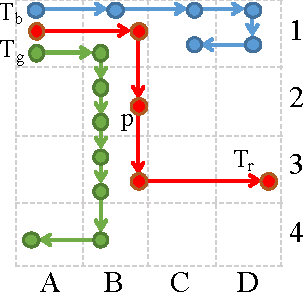
\includegraphics[scale=.6]{patterns2.pdf}
    \caption{Trajectories moving through a tessellation.}
    \label{fig:patterns2}
\end{figure}

\begin{example}[Trajectory and transaction]
With reference to \Cref{fig:patterns2}, 
% where a regular tessellation is used for simplicity, 
$T_b,T_g$, and $T_r$ are trajectories while $Q_{A1}$ and $Q_{B2}$ are transactions that correspond to tiles A1 and B2.
{\small
\begin{align*}
    T_b&= (A1, B1, C1, D1, C1),
    T_g = (A1, B1, B2, B3, B4, A4),\\
    T_r&= (A1, B1, B2, B3, D3),Q_{A1}=\{T_b, T_g, T_r \},Q_{B2}= \{T_g, T_r \}
\end{align*}
}
% \noindent Mapping $T_g$ into the tessellation allows its compression since consecutive points in tiles $B2$ and $B3$ are only stored once. 
% The tessellation defines the granularity and the semantics of the analysis.
% If --- for instance --- the user is also interested in distinguishing malls or restaurants or means of transport, space and time features alone are not enough.
% Additional features (e.g., placeType or transport) must be added to the tessellation.
% This is the strength of our approach: to consider custom features transparently.
% Indeed, tiles enable an extensible and transparent management of space, time, and additional features.
% For instance, in a 2D setting (where only space --- latitude and longitude --- is considered), tiles $A1$ and $A2$ could represent the following bins/partitions 
% {\small
% \begin{align*}
% A1 = (lat=44.123, lon=12.123)\\
% B2 = (lat=44.124, lon=12.124)   
% \end{align*}}
% \noindent while in a 4D setting (space, time, and means of transport) $A1,A2$ could be
% {\small
% \begin{align*}
% A1 = (&lat=44.123, lon=12.123, t=2022/08/04~10:55:00, transport=walk)\\
% B2 = (&lat=44.124, lon=12.124, t=2022/08/04~10:56:00, transport=bus)
% \end{align*}}
\end{example}
%
% While this modeling naturally allows the extraction of groups of trajectories moving in defined spatial regions, some might find more natural to do a ``transposed'' modeling using tiles as items and trajectories as transactions.
% In this case, the output would be the groups of places traveled by multiple trajectories rather than the group of trajectories traveling multiple places.
% In this case, the output would be the groups of places visited together rather than the group of trajectories traveling together.
% However, 
% A frequent itemset would be composed of a set of tiles that are often crossed together, while the reference to the trajectories, which is the real objective of the analysis, would be lost.
 
The maximum number of transactions depends on the number of tiles (i.e., $|\mathcal{Q}| = |S|$).
Modeling trajectories as items and tiles as transactions makes our frequent itemset approach a \textit{colossal} one since the number of tiles (i.e., transactions) is typically in the order of magnitudes smaller than the number of trajectories (i.e., items). 
This is a fair assumption to make: for instance, Milan has 88 neighborhoods with over $3 \cdot 10^6$ inhabitants (i.e., potential MOs). 
Obviously, our assumption is no more true when a very fine tessellation is adopted.
For example, the Milan metropolitan area spans about $1500km^2$, corresponding to $1.5\cdot10^5$ uniform tiles with side $100m$ and $1.5\cdot10^7$ uniform tiles with side $10m$.
% \begin{figure}
%     \centering
%     \includegraphics[scale=.6]{complexity4.pdf}
%     \caption{Given a dataset of trajectories $\mathcal{R}$ the number of possible groups/clusters $2^{|\mathcal{R}|}$. However, when the goal is to extract trajectories moving in $S$ regions (e.g., $|S|=100$), the number of possible groups/clusters becomes $2^{|S|}$ independently of the number of trajectories; the fewer the regions the narrower the search space.}
%     \label{fig:complexity}
% \end{figure}

\subsection{Mining co-movement patterns}
We retrieve the sets of trajectories satisfying minimum cardinality (i.e., the number of trajectories), minimum support (i.e., the length of the shared path), and spatio-temporal constraints.
Different mobility patterns can be obtained by specializing such constraints.% (as later shown).

\begin{definition}[Co-movement pattern]\label{def:comov}
A \textit{co-movement pattern} $I$ is a FCI s.t. $|I| \ge mCrd$, where $mCrd$ is the minimum number of trajectories to consider a FCI as a co-movement pattern.
\end{definition}

% By definition, a co-movement pattern has at least $mCrd$ trajectories and is at least $mSup$ tiles long.
This ``basic'' co-movement pattern can be specialized 
%into those reported in \Cref{tab:proximitypattern} 
depending on the involved features.
% , either space ($f^{sp}$) or space and time ($f^{tm}$), and on the additional shape constraints described in \Cref{tbl:constraints2}.
% \Cref{fig:allpatterns} depicts an example of each pattern.
\begin{table}[t]
\caption{Characterization of co-movement patterns}% in terms of spatial ($f^{sp}$) and temporal ($f^{tm}$) features and shape constraints}
\label{tbl:constraints2}
\scriptsize\centering
\begin{tabular}{lcl}
\toprule
Pattern     & Feature         & Shape constraints \\
\midrule
Co-loc. &$f^{sp}$             & None \\
Flow        &$f^{sp}$             & \specialcell{$\exists S' \subseteq sup(I)$ s.t.~ $\forall s_i,s_j \in S', s_i\leftrightarrow_{f^{sp}} s_j \wedge |S'|\geq mSup$}\\
Swarm       &$f^{sp}, f^{tm}$         & None \\
Convoy      & $f^{sp}, f^{tm}$ & \specialcell{$\exists S' \subseteq sup(I)$ s.t.~  $\forall s_i,s_j \in S', s_i\leftrightarrow_{f^{tm}} s_j \wedge |S'|\geq mSup$}\\
\bottomrule
\end{tabular}%
\end{table}
% \begin{enumerate}[label=(\alph*)]
%     \item Co-location \citep{DBLP:journals/isci/FranciaGR20}: trajectories sharing spatial points (e.g., individuals working and shopping in the same places, even at different times). No shape constraint is needed and the tessellation must include the space feature.
%     \item Flow \citep{DBLP:journals/tmc/HanLO15}: trajectories sharing \textit{contiguous} spatial points (e.g., traffic over contiguous roads).
%     The shape constraint ensures tile connection on the space dimension.
%     \item Swarm \citep{DBLP:journals/pvldb/LiDHK10}: trajectories sharing spatial points at the same time (e.g., individuals being occasionally together). No shape constraint is needed and the tessellation must include space and time features.
%     % \item Platoon \citep{DBLP:journals/dke/LiBK15}: trajectories sharing spatial points for at least $mSup$ continuous time intervals (e.g., individuals sharing a means of transport for some time). The constraint ensures time continuity for each sub-pattern. A platoon can include several time-continuous sub-patterns. 
%     \item Convoy \citep{DBLP:journals/pvldb/JeungYZJS08}: trajectories sharing spatial points \textit{continuously} in time (e.g., individuals moving together\footnote{While the original formalization involves individuals \textit{always} moving together, this constraint has been relaxed to a \textit{sufficient} amount of contiguous temporal tiles \citep{DBLP:journals/pvldb/FanZWT16}. Otherwise, meaningful patterns can be lost due to noisy trajectories (even a single missing trajectory point).}). The shape constraint ensures tile connection on the time dimension.
% \end{enumerate}
% As summarized in \Cref{tbl:constraints2}, 
Co-location and flow are defined over a spatial feature ($f^{sp}$; i.e., they are required to happen in the same spatial tile), while swarm and convoy require both spatial ($f^{sp}$) and temporal ($f^{tm}$) features (i.e., they are required to happen in the same spatio-temporal tiles).
In other words, while for swarm and convoy it is necessary to be in the same spatio-temporal tile, co-location and flow only require to be in the same spatial tile (e.g., same location even if at different times).
% A strong point of CTM is the capability to homogeneously manage space, time, and any additional semantic feature.

Although the simplest representation of the space and time features is a regular binning of their absolute values, CTM allows adopting abstractions richer in semantics as long as these determine a tessellation (i.e., a partitioning) of space and time.
%For example, space can be partitioned into neighborhoods or regions, while time can be arranged in a finite set of categorical values such as holidays-working days, morning-afternoon-night, and so on. 
%
% \subsection{Handling additional features through behavioral constraints}
% \label{sec:constr}
% Co-movement patterns are described by more than space and time features alone.
% Nominal, ordinal, and continuous features can further characterize behaviors that trajectories must share.
% Individuals could share means of transport and activities, or move and stand together; for instance, groups of people can take the same means of transport to reach the city center and go shopping in the same malls.
% To create a co-movement pattern, feature values must be the same in the path shared by the MOs (e.g., to be in the same group, individuals should share the same means of transport).
%
Characterizing co-movement patterns with additional features means imposing additional constraints, which we call \textit{behavioral} constraints. 
Note that behavioral constraints are more expressive than filtering trajectories based on a specific feature value since they further characterize objects that \textit{behaves similarly} while moving in space and time; for instance, behavioral features are highly important in the linkage/anonymization of mobility data \citep{DBLP:journals/tkde/JinHFCOZ23}.
In CTM, behavioral constraints are transparently enforced by simply extending the input tessellation with additional features (see \Cref{def:tes}, the tile directly models the features in the tessellation).
More formally, two or more trajectories \textit{share} a tile $s$ if they have at least a point in $s$. Then, the support of an itemset $I$ (a set of trajectories), includes all and only the transactions (tiles) shared by the trajectories.
Note that the behavioral constraints must be computed jointly with the spatio-temporal ones, and not before/after running CTM.
% \begin{itemize}
%     \item A \textit{pre-processing strategy} could apply behavioral constraints directly to the raw trajectory dataset (i.e., before applying CTM). 
%     At this stage, only filters on single trajectories can be applied.
%     However, behavioral constraints require the portion of space/time shared by groups of trajectories to be known. 
%     % The need of knowing this information (carried by tiles) makes it impossible to apply constraints in the pre/post-processing phase unless requiring further computations.
%     \item A \textit{post-processing strategy} could compute co-movement patterns considering spatio-temporal features first and then discarding the returned co-movement patterns that do not fulfill behavioral constraints.
%     However, co-movement patterns are closed by definition.
%     If a co-movement pattern becomes unfeasible due to behavioral constraints some of its non-closed subsets will become closed and must be returned. 
%     Since only closed itemsets are computed and returned, closeness and feasibility should be tested for all the subsets; however, the cardinality of the subsets is exponential in the pattern support.
%     Alternatively, an approach returning non-closed itemsets too should be adopted, but this would imply much heavier enumeration \citep{DBLP:journals/tkde/LuccheseOP06}. 
% \end{itemize}
% \begin{example}
% Suppose we are looking for co-location patterns (i.e., individuals moving through some places without time constraints) characterized by stop-move phases, where stop points are used to infer the purpose of a trip and moves can provide information such as direction and mode of transport \citep{DBLP:journals/tgis/WangM18}.
% Let $mSup=3$ and consider three individuals Alice, Charles, and Paul sharing the same route of 3 tiles $A1,B1$, and $C1$.
% %On the one hand, Alice and Charles stop by stores in tiles $A1$ and $C1$ and walk by $B1$. On the other hand, Paul is walking through the three tiles. Thus, given $mSup=3$, we want only $\{Alice, Charles\}$ to emerge as a co-movement pattern.
% On the one hand, Alice and Charles stop by stores in tiles $A1$ and $C1$ and walk by $B1$. On the other hand, Paul is only walking through the three tiles. Thus, considering the speed feature, only $\{Alice, Charles\}$ should emerge as a co-movement pattern, while $\{Alice, Charles, Paul\}$ (which is valid only from the spatio-temporal point of view) should be discarded.
% A pre-processing technique could be to discretize speed values and run an instance of CTM for each speed bin value; however, the pattern related to $\{Alice, Charles\}$ would be lost since it involves \textit{both} walking and stops; more formally, $sup(\{Alice, Charles\})=|\{Q_{B1}\}|<mSup$ when walking and $sup(\{Alice, Charles\})=|\{Q_{A1},Q_{C1}\}|<mSup$ when shopping.
% Alternatively, a post-processing technique could be to run CTM with only spatio-temporal features, return both $\{Alice, Charles, Paul\}$ and $\{Alice, Charles\}$, and finally discard the former by analyzing the speed feature. However, since $sup(\{Alice, Charles, Paul\})=sup(\{Alice, Charles\})$, the pattern $\{Alice, Charles\}$ is not closed (see \Cref{def:fci}) and cannot be returned; as result, the valid co-movement pattern $\{Alice, Charles\}$ is lost.
% \end{example}

% \begin{figure}[t]
%     \begin{subfigure}[t]{.5\columnwidth}
%         \centering
%         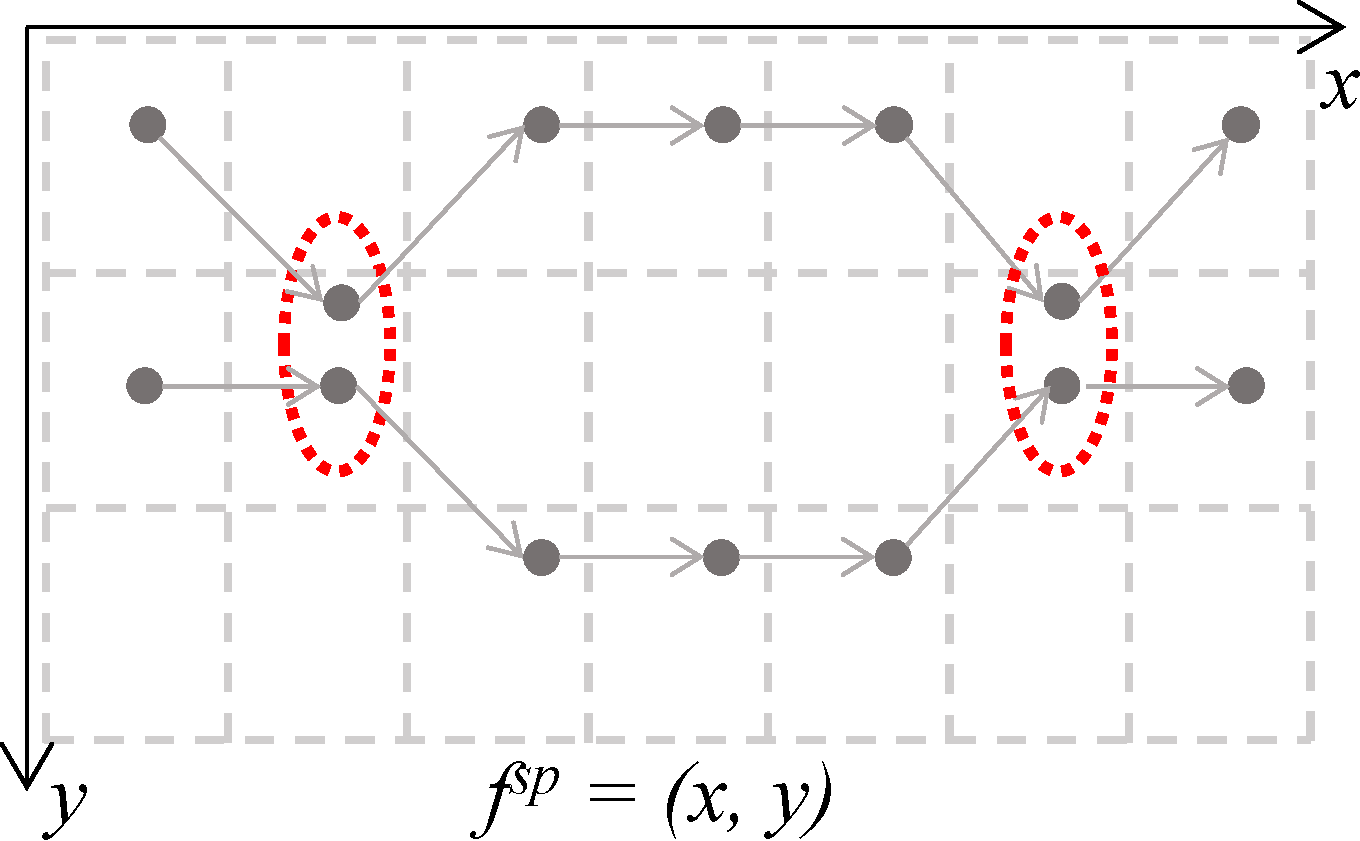
\includegraphics[scale=.18]{colocation.pdf}
%         \caption{Co-location ($mSup=2$)}
%         \label{fig:colocation}
%     \end{subfigure}~
%     \begin{subfigure}[t]{.5\columnwidth}
%         \centering
%         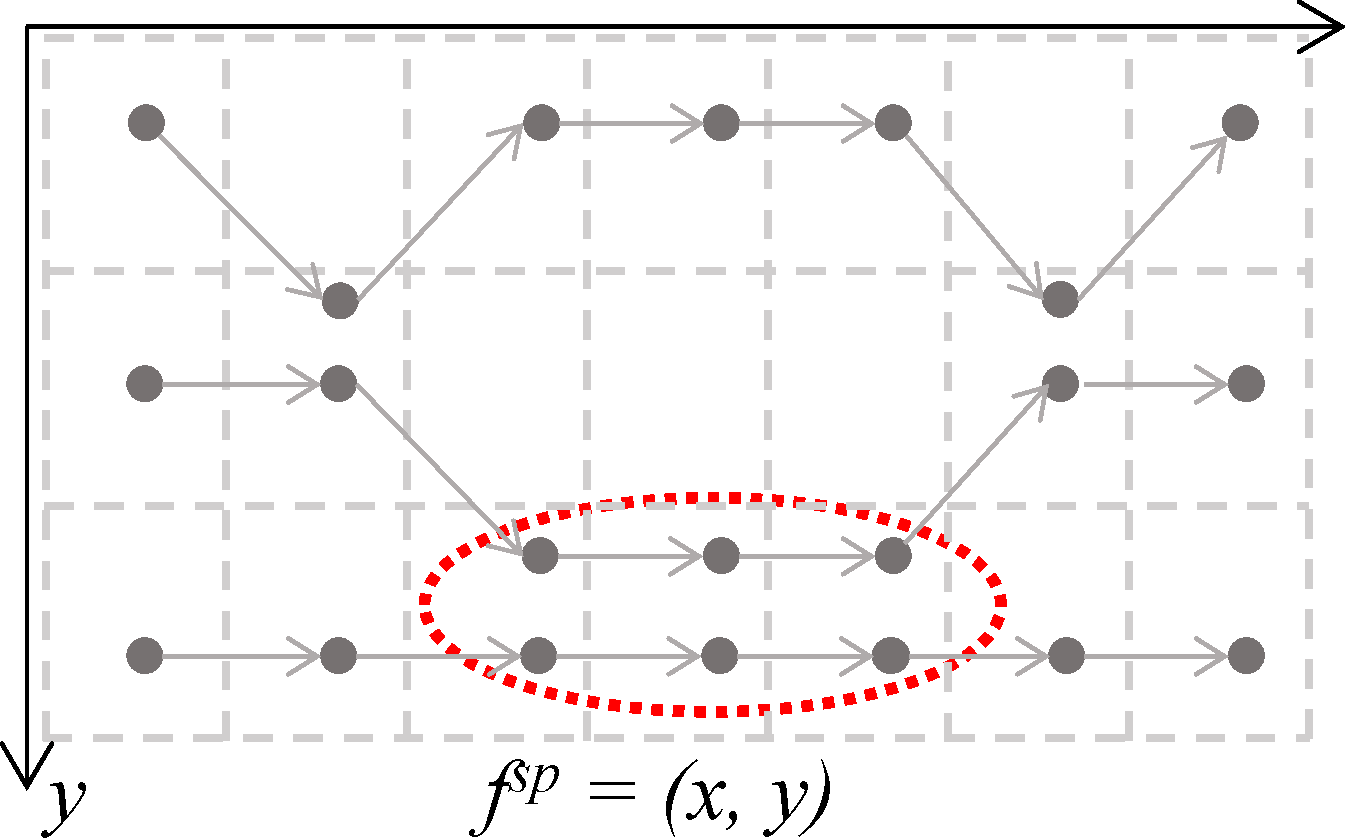
\includegraphics[scale=.18]{flow.pdf}
%         \caption{Flow ($mSup=3$)}
%         \label{fig:flow}
%     \end{subfigure}
%     \\
%     \begin{subfigure}[t]{.53\columnwidth}
%         \centering
%         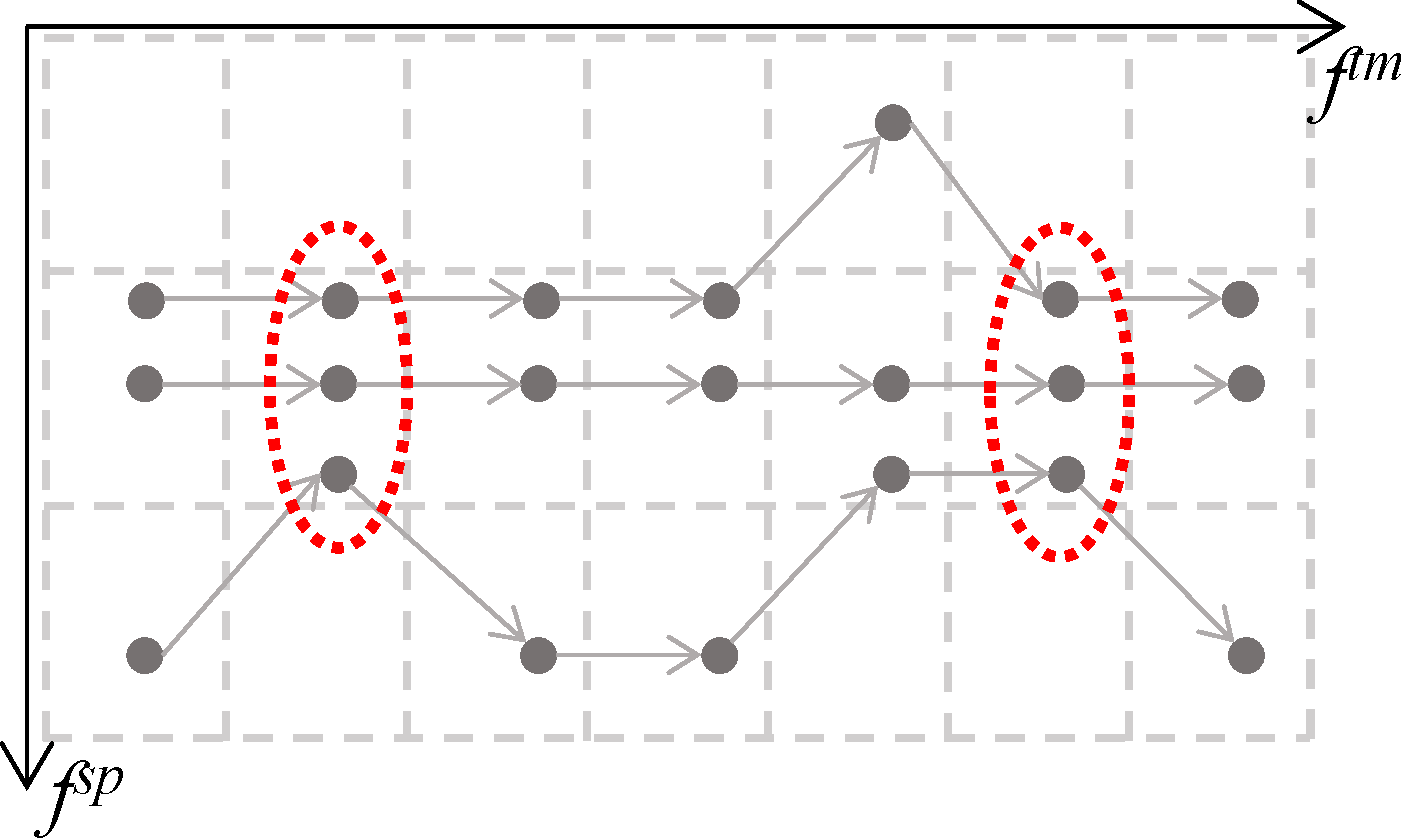
\includegraphics[scale=.18]{swarm.pdf}
%         \caption{Swarm($mCrd=3,mSup=2$)}
%         \label{fig:swarm}
%     \end{subfigure}~
%     % \begin{subfigure}[t]{.5\columnwidth}
%     %     \centering
%     %     \includegraphics[scale=.65]{platoon.pdf}
%     %     \caption{Platoon ($mSup=2$)}
%     %     \label{fig:platoon}
%     % \end{subfigure}\\
%     \begin{subfigure}[t]{.5\columnwidth}
%         \centering
%         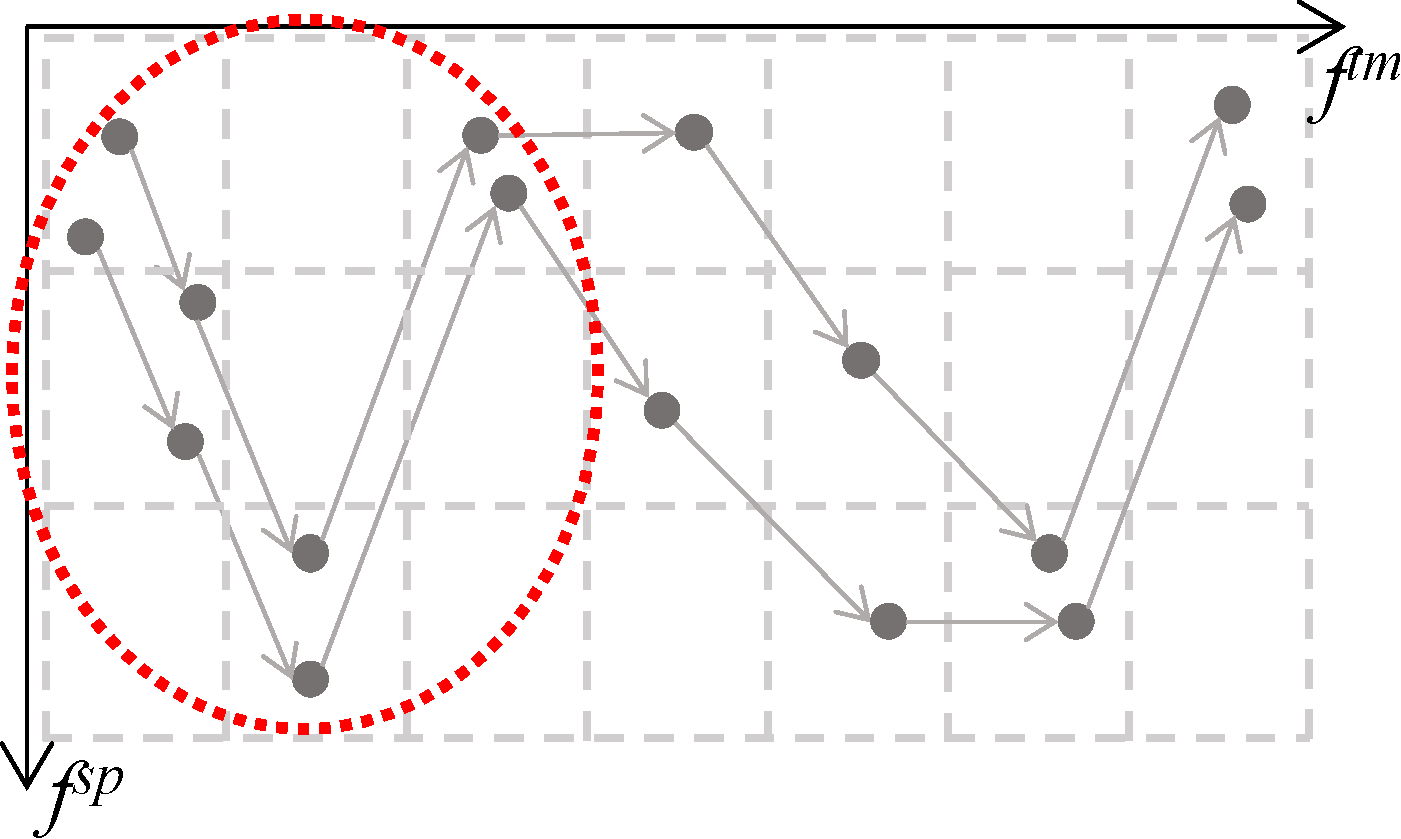
\includegraphics[scale=.18]{flock.pdf}
%         \caption{Convoy ($mSup=4$)}
%         \label{fig:flock}
%     \end{subfigure}
%     \caption{Co-movement patterns (unless specified, $mCrd=2$).}
%     \label{fig:allpatterns}
% \end{figure}

% We initially remind that trajectories are mapped to items and tiles are mapped to transactions.
% For the sake of clarity, henceforth we only refer to the items and transactions.

When the number of items is much larger than the number of transactions, searching for frequent itemsets by enumerating all itemsets with an \textit{Apriori-like strategy} \citep{DBLP:conf/vldb/AgrawalS94} can be unfeasible or very inefficient.
In this case, it is convenient to adopt a \textit{row-enumeration-like strategy} \citep{DBLP:conf/kdd/PanCTYZ03}. %, which is enumerating all the possible transaction sets.
% Each set of transactions $\bar{\mathcal{Q}}$ corresponds to the intersection of the itemsets appearing in those transactions.
%
% \begin{definition}[$\bar{\mathcal{Q}}$-Itemset]
% Given a transaction dataset $\mathcal{Q}$, a \textit{$\bar{\mathcal{Q}}$-itemset} is the largest itemset supported by all transactions $\bar{\mathcal{Q}} \subseteq \mathcal{Q}$.
% \end{definition}
% Each transaction corresponds to a $\bar{\mathcal{Q}}$-itemset with $|\bar{\mathcal{Q}}|=1$; a generic $\bar{\mathcal{Q}}$-itemset is the intersection of the itemsets in $\bar{\mathcal{Q}}$.
% \begin{example}[$\bar{\mathcal{Q}}$-Itemset]
% With reference to \Cref{fig:patterns2}, $I = \{T_g,T_r\}$ is a $\bar{\mathcal{Q}}$-itemset with $\bar{\mathcal{Q}}=\{Q_{A1},Q_{B1},Q_{B2},Q_{B3}\}$.
% \end{example}
% \begin{theorem}[Closeness of $\bar{\mathcal{Q}}$-itemset]
% $\bar{\mathcal{Q}}$-itemsets are all and only the closed itemsets.
% \end{theorem}
% The proof is available in the extended version.
% See \Cref{ap:t1} in \ref{ap:proof}.
%
CTM extracts co-movement patterns through a breadth-first enumeration of 
%$\bar{\mathcal{Q}}$-
closed itemsets: starting from single transactions, CTM progressively intersects them with further transactions.
% $\bar{\mathcal{Q}}$-
Closed itemsets associated with a larger set of transactions are characterized by lower cardinalities and larger supports (intuitively, fewer trajectories sharing more tiles).
The enumeration process can be represented as an enumeration tree, where each node 
%$N$ 
corresponds to a distinct closed itemset.
% set of transactions $\bar{\mathcal{Q}}$.
% We call \textit{enumeration sequence} the path leading from the root to a node $N$.
Naively enumerating the whole tree is inefficient, thus we exploit several pruning mechanisms to limit the enumerated portion of the tree.
We conceive CTM as a parallel and big-data approach for co-movement pattern mining.
%, thus it exploits solutions that would be neither necessary nor optimal in a centralized implementation.
Specifically, CTM:
% \begin{itemize}
% \item 
(i) adopts a breadth-first enumeration approach to fully exploit task parallelization and workload balancing;
% \item 
(ii) adopts local pruning criteria to avoid centralized checks that would limit parallelization;
% \item 
(iii) adopts spatio-temporal pruning criteria that have been specifically devised for trajectories-related patterns;
% \item 
(iv) broadcasts the transaction dataset %$\mathcal{Q}$ 
to locally compute the itemset support.
% This is a reasonable assumption since following our approach, its size is limited and can fit the central memory (see \Cref{sec:test}).
% \end{itemize}
For the sake of space, the details of the enumeration process are omitted and are available in the extended version \cite{DBLP:journals/eswa/FranciaGG24}.

Note that approaching this problem as a colossal itemset mining rather than a typical clustering one 
% \begin{itemize}
    % \item 
(i) avoids the computation of similarities that would make computational complexity explode for large datasets;
and (ii) exploits monotonicity properties (e.g., as the generation process proceeds, the cardinality of trajectory groups decreases while the length of the path shared by trajectories in the same group increases) to filter out invalid co-movement patterns without generating them all.
%(filtering strategies are detailed in \Cref{sec:pruning}).
% \end{itemize}

% We now introduce the enumeration process, the pruning techniques, and, finally, how we distribute the algorithm to support scalable generation of co-movement patterns.

% \subsection{The enumeration process}
% \Cref{alg:colossal} introduces the pseudo-code of CTM which takes as inputs the transaction dataset $\mathcal{Q}$, the minimum cardinality $mCrd$, and the minimum support $mSup$.
% For the sake of simplicity, we assume $\mathcal{P}$ (Line \ref{alg:col01}) to be a \textit{global} variable used as an accumulator of nodes corresponding to the co-movement patterns to be returned.
% $\mathcal{L}$ (Line \ref{alg:col01bis}) is a first-in-first-out (FIFO) queue that ensures breadth-first enumeration.
% We use the ``dot'' notation to indicate the information in each node $N$.
% Each enumeration node $N$ is associated with a $\bar{\mathcal{Q}}$-itemset $N.I$.
% Such $\bar{\mathcal{Q}}$-itemset is obtained by intersecting the transactions building up the enumeration sequence $N.CT$ (\textit{Covered Transactions}), which is $N.CT=\bar{\mathcal{Q}}$.
% Let $ N.RT $ (\textit{Remaining Transactions}) be the transactions whose enumeration is expected in the $N$ subtree.
% Note that enumeration nodes are unique: they can lead to the same itemset $N.I$ but they will have different $N.CT$ and $N.RT$.
% Nodes that potentially contain co-movement patterns are added to the queue (Line \ref{alg:col07}).
% While at least an extendable node exists (Line \ref{alg:col08}), a node is removed from the queue (Line \ref{alg:col09}) and extended (Line \ref{alg:col10-bis}); the resulting nodes are appended in $\mathcal{L}$ (Line \ref{alg:col10}).
% Finally, the nodes associated with co-movement patterns are returned (Line \ref{alg:colret}).

% \begin{algorithm}[t]
% \caption{CTM}\label{alg:colossal}
%  \scriptsize\centering
% \begin{algorithmic}[1]
% \Require $\mathcal{Q}$: transactions, $mSup$: minimum support, $mCrd$: minimum cardinality%, $S$: tessellation
% \Ensure $\mathcal{P}$: co-movement patterns
% % \State Broadcast $\mathcal{Q}$ \Comment{Make $\mathcal{Q}$ available to distributed executors}
% \State $\mathcal{P} \gets \varnothing$ \Comment{Global accumulator of co-movement patterns}                              \label{alg:col01}
% \State $\mathcal{L} \gets \varnothing$ \Comment{FIFO queue of $\bar{\mathcal{Q}}$-itemsets}                                      \label{alg:col01bis}
% \ForEach{$Q \in \mathcal{Q}$} \Comment{For each transaction}
%     \State $N \gets newNode()$ \Comment{create an enumeration node}    \label{alg:col02}     \State $N.I \gets Q$ \Comment{initialize the node $\bar{\mathcal{Q}}$-itemset with a transaction}                                                         \label{alg:col03-bis}
%     \State $N.CT \gets \{ Q \}$ \Comment{set the Covered Transactions}                                         \label{alg:col03}
%     \State $N.RT \gets \{ Q' | Q' \in \mathcal{Q}, id(Q') > id(Q) \}$ \Comment{set the Remaining Transactions} \label{alg:col04}
%     \State $\mathcal{L}.enqueue(N)$ \Comment{enqueue the node for extension} \label{alg:col07} 
% \EndFor
% \While{$|\mathcal{L}|>0$}\Comment{While an extendable node exists}                                 \label{alg:col08}
%         \State $N \gets \mathcal{L}.dequeue $ \Comment{remove it from the queue}                          \label{alg:col09}
%         \State $\bar{\mathcal{L}} \gets Extend(N,mSup,mCrd)$ \Comment{extend it} \label{alg:col10-bis}
%         \State $\mathcal{L}.enqueue(\bar{\mathcal{L}})$ \Comment{add the new nodes to the queue}       \label{alg:col10}
% \EndWhile
% \State \Return $\mathcal{P}$ \Comment{Return the co-movement patterns}             \label{alg:colret}
% \end{algorithmic}
% \end{algorithm}

% \Cref{alg:extend}, applied in \Cref{alg:colossal} Line \ref{alg:col10-bis}, shows how enumeration nodes are extended.
% First of all, if the node corresponds to a valid co-movement pattern (Line \ref{alg:ext02}), it is added to the global accumulator (Line \ref{alg:ext04}).
% Then, an empty queue is initialized to store the extendable nodes (Line \ref{alg:ext01}), which are enumerated by $N$ if the latter can potentially generate co-movement patterns (Line \ref{alg:ext15}).
% The $Check()$ function, which verifies validity and extensibility of a pattern, is discussed in \Cref{sec:pruning}.
% Before enumerating new nodes, Lines \ref{alg:ext05}-\ref{alg:ext07} avoid useless extension steps: transactions $Y$ shared by all the items in the $\bar{\mathcal{Q}}$-itemset (Line \ref{alg:ext05}) will generate no new $\bar{\mathcal{Q}}$-itemsets since intersecting $N.I$ with the transactions in $Y$ would produce $N.I$ itself by definition.
% Thus, transactions in $Y$ should not be intersected; they can be removed from $N.RT$ and directly added into $N.CT$.
% For each of the transactions that have yet to be covered (Line \ref{alg:ext10}), a new node is generated by intersecting the items in $N.I$ with the ones in the transaction (Line \ref{alg:ext11}).
% The transaction is then added to the covered ones (Line \ref{alg:ext12}) and consequently removed from $RT_{next}$ (Line \ref{alg:ext13}) which is assigned to the new node as the set of remaining transactions (Line \ref{alg:ext14}).
% Finally, the current node is queued for extension (Line \ref{alg:ext17}).
% When the entire set of remaining transactions is exhausted, the extended nodes potentially entailing co-movement patterns are returned (Line \ref{alg:extret}).

% \begin{algorithm}[t]
% \caption{Extend}\label{alg:extend}
% \scriptsize\centering
% \begin{algorithmic}[1]
% \Require $N$: enumeration node, $mSup$: support, $mCrd$: cardinality
% \Ensure $\mathcal{L}$: Extended $\bar{\mathcal{Q}}$-itemsets
% \If {$Check(N,\text{``val''},mSup,mCrd) = true$}\label{alg:ext02}
%     \item[] \Comment{If $N$ refers to a co-movement pattern}
%     \State $\mathcal{P} \gets \mathcal{P} \cup \{N\}$ \Comment{store it}\label{alg:ext04}
% \EndIf
% \State $\mathcal{L} \gets \varnothing$ \Comment{Initialize a node queue}                                            \label{alg:ext01}
% \If{$Check(N,\text{``ext''},mSup,mCrd) = true$} \label{alg:ext15}
%     \item[] \Comment{If $N$'s subtree potentially contains co-movement patterns}
%     \State $Y \gets sup(N.I) \cap N.RT$ \Comment{Transactions shared by all items in $N.I$}                           \label{alg:ext05}
%     \State $N.CT \gets N.CT \cup Y$ \Comment{are added to the covered set}                                        \label{alg:ext06}
%     \State $N.RT \gets N.RT \setminus Y$ \Comment{and removed from those to be extended}                             \label{alg:ext07}
%     \State $RT_{next} \gets N.RT$ \Comment{Initialize $RT_{next}$}                        \label{alg:ext07bis}
%     \ForEach{$Q \in N.RT$} \Comment{For each remaining transaction}                                             \label{alg:ext10}
%         \State $N' \gets newNode()$ \Comment{create an enumeration node $N'$}\label{alg:ext10b}
%         \State $N'.I \gets N.I \cap Q$ \Comment{set the $\bar{\mathcal{Q}}$-itemset}                                        \label{alg:ext11}
%         \State $N'.CT \gets N.CT \cup \{ Q \}$ \Comment{extend the Covered Transactions}                             \label{alg:ext12}
%         \State $RT_{next} \gets RT_{next} \setminus \{ Q \}$ \Comment{reduce the Remaining Transactions} \label{alg:ext13}
%         \State $N'.RT \gets RT_{next}$ \Comment{and assign them to $N'$}                                          \label{alg:ext14}
%         \State $\mathcal{L}.enqueue(N')$ \Comment{enqueue the node for extension}                                 \label{alg:ext17}
%     \EndFor
% \EndIf
% \State \Return $\mathcal{L}$ \Comment{Return the extended nodes} \label{alg:extret}
% \end{algorithmic}
% \end{algorithm}

% \begin{algorithm}[t]
% \scriptsize\centering
% \caption{Check}\label{alg:filterE}
% \begin{algorithmic}[1]
% \Require $N$: enumeration node, $type$: type of check (either ``val'' for validity, or ``ext'' for extensibility), $mSup$: support, $mCrd$: cardinality
% \Ensure Whether the node satisfies the constraints
% \State $validCrd \gets |N.I| \ge mCrd$ \Comment{Cardinality check}  \label{alg:filterE1} 
% \State $nonRed \gets sup(N.I) = N.CT$ \Comment{Redundancy check} \label{alg:filterE3}
% \If{$type = \text{``val''}$}
%     \State $validSup \gets IsSupported(N.CT, mSup)$ \Comment{Support
%     and shape check}  \label{alg:filterE2Val}
% \ElsIf{$type = \text{``ext''}$}
%     \State $validSup \gets IsSupported(N.CT \cup N.RT, mSup)$ \label{alg:filterE2Ext}
%     \item[] \Comment{Support and shape check on the best hypothesis of $N$'s subtree}  
% \EndIf
% \State \Return $ validCrd \wedge nonRed \wedge validSup$ 
% \end{algorithmic}
% \end{algorithm}

% \begin{figure}[t]
% \begin{subfigure}{.48\columnwidth}
%     \centering
%     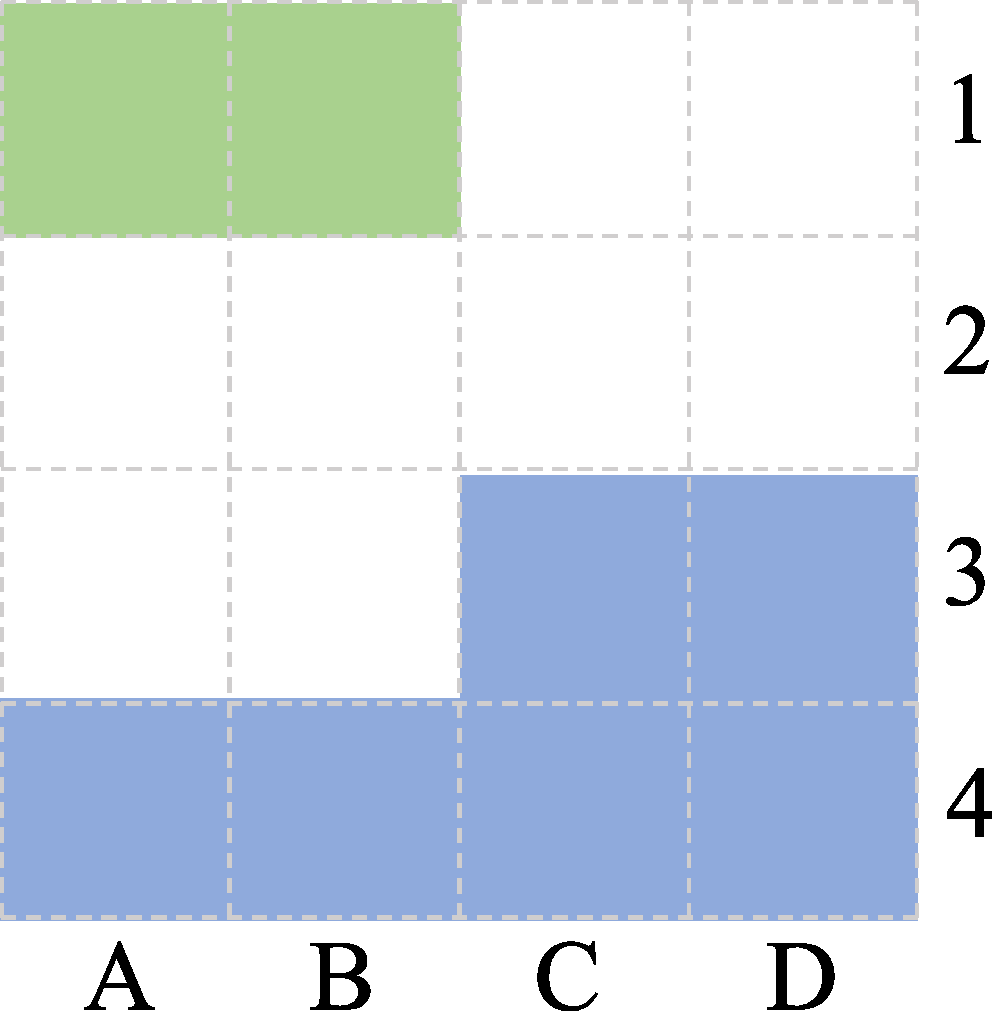
\includegraphics[scale=.18]{pruning.pdf}
%     \caption{(Un)connected components.}
%     \label{fig:conncomp}
% \end{subfigure}
% \begin{subfigure}{.48\columnwidth}
%     \centering
%     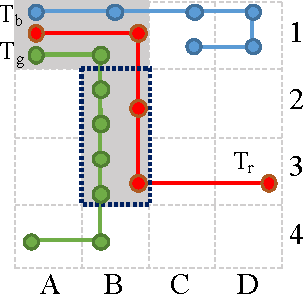
\includegraphics[scale=.6]{theorem.pdf}
%     \caption{Redundancy.}
%     \label{fig:theorem}
% \end{subfigure}
% \caption{Shape and redundancy checks}
% \end{figure}

% \subsection{Validity check and enumeration pruning} \label{sec:pruning}
% CTM relies on three different checks to validate co-movement patterns and to prune subtrees.
% Checks are implemented through the $Check()$ function.

% \textbf{Cardinality check}.
% This check verifies whether the $\bar{\mathcal{Q}}$-itemset comprises enough items (i.e., trajectories).
% The minimum cardinality is necessary to validate a pattern.
% Additionally, since it holds the anti-monotone property, it can be used to prune $N$'s subtree as well.
% In particular, an itemset's cardinality monotonically decreases with extensions since itemsets related to nodes in $N$'s subtree are obtained by intersecting $N.I$ with additional transactions (see \Cref{alg:extend} Line \ref{alg:ext11}).
% Thus, if a $\bar{\mathcal{Q}}$-itemset $N.I$ does not fulfill the cardinality constraint, none of its extensions will, and $N$'s subtree can be pruned.

% \textbf{Support and shape check}.
% This check verifies the minimum support and the connection constraints as in \Cref{tbl:constraints2}.
% The check relies on the $IsSupported(\mathcal{Q}^*,mSup)$ function, which takes in input a set of transactions $\mathcal{Q}^*$ and carries out different checks according to the searched pattern type.
% \begin{itemize}
% \item \textit{Co-location} and \textit{Swarm} patterns do not require shape constraints but only sufficient support ($|\mathcal{Q}^*|\geq mSup$).
% \item \textit{Flow} and \textit{Convoy} patterns require tiles to be connected.
% This can be checked by verifying if, in $|\mathcal{Q}^*|$, there are transactions corresponding to two tiles connected by a path long at least $mSup$ (see \Cref{def:adj}).
% Obviously, if such a connected pair exists, the minimum support constraint is fulfilled too.
% In our context, the tessellation fits the main memory of every single machine, thus connected components can be found in linear time \citep{hopcroft1973algorithm}.
% \end{itemize}

% Additionally to the shape check discussed above, the $IsSupported()$ function also verifies the minimum support.
% Notice that this verification is different, depending on whether the pattern is checked for \textit{validity} or for \textit{extensibility} (\Cref{alg:filterE} Lines \ref{alg:filterE2Val} and \ref{alg:filterE2Ext}, respectively).
% Validity is verified on the current pattern's covered transactions, i.e., $\mathcal{Q}^* = N.CT$.
% To verify extensibility, we must consider that (differently from cardinality) support and shape hold the monotonic property (as $CT$ is always incremented with new transactions): if a $\bar{\mathcal{Q}}$-itemset does not fulfill the support and shape constraint, some of its extensions can.
% Thus, the pruning of $N$'s subtree is possible only by verifying that none of the nodes in $N$'s subtree satisfies these constraints.
% An exact verification would require to enumerating all the nodes in the subtree to generate the corresponding $\bar{\mathcal{Q}}$-itemsets (which is exactly what we want to avoid).
% We optimize this verification by considering $\mathcal{Q}^* = N.CT \cup N.RT$ as a \textit{best hypothesis}, i.e., an optimistic transaction layout that includes all the transactions in the $N$'s subtree.
% Even if it has not been verified whether a corresponding $\bar{\mathcal{Q}}$-itemset exists, it serves as an upper-bound to the support and shape check, thus allowing $N$'s subtree to be pruned if the best hypothesis does not pass the check.

% \begin{example}
% With reference to \Cref{fig:conncomp}, given $I.CT=\{Q_{A1},Q_{B1}\}$ (green) and $I.RT=\{Q_{C3},\ldots,Q_{D4}\}$ (blue), $I.CT \cup I.RT$ cannot produce a convoy with $mSup=7$ (there are no 7 adjacent tiles) but can potentially produce a convoy with $mSup=6$ (there are 6 adjacent --- blue --- tiles).
% \end{example}

% \textbf{Redundancy check}.
% This check avoids generating a $\bar{\mathcal{Q}}$-itemset more than once.
% The enumeration strategy relies on transaction lexicographic ordering (\Cref{alg:colossal} Line \ref{alg:col04}) to perform a systematic and non-redundant enumeration of transaction combinations.
% Nonetheless, the same $\bar{\mathcal{Q}}$-itemset $I$ could result from two different sets of transactions $S'$ and $S''$.
% We rely on the $\bar{\mathcal{Q}}$-itemset redundancy definition below to prune the enumeration tree.

% \begin{definition}[Non-redundant enumeration node]
% An enumeration node $N$ is non-redundant if $sup(N.I) = N.CT$.
% \end{definition}

% \begin{example}[Redundancy]
% \label{ex:redundancy}
% With reference to \Cref{fig:theorem}, let $N$, $N'$ and $N''$ be enumeration nodes.
% Let $N.I=\{T_g,T_r\}$ be a $\bar{\mathcal{Q}}$-itemset with $sup(N.I)=\{Q_{A1},Q_{B1},Q_{B2},Q_{B3}\}$ (gray area).
% The $\bar{\mathcal{Q}}$-itemset can be generated by intersecting $N'.I=\{T_b,T_g,T_r\}$ (with $N'.CT=\{Q_{A1},Q_{B1}\}$ and $N'.RT=\{Q_{C1},\ldots,Q_{D4}\}$) with the transaction $Q_{B2}=\{T_g,T_r\}$.
% Alternatively, it can be obtained directly from $Q_{B2}$, where $N''.I=Q=\{T_g,T_r\}$ with $N''.CT=\{Q_{B2},Q_{B3}\}$ (dotted area) and $N''.RT=\{Q_{C2},\ldots,Q_{D4}\}$.
% $N''$ will be discarded since redundant, i.e. $N''.CT \subset sup(N''.I)=sup(N.I)$.
% Note that, even if $N''$ refers to transaction $Q_{B2}$, $N''.CT$ is automatically extended to $\{Q_{B2},Q_{B3}\}$ by \Cref{alg:extend} Line \ref{alg:ext06}.
% \end{example}


% \begin{theorem}[Uniqueness of non-redundant enumeration nodes]
% There do not exist two distinct non-redundant enumeration nodes $N$ and $N'$ such that $N.I=N'.I$.
% \end{theorem}
% See \Cref{ap:t2} in \ref{ap:proof}.

% Dropping redundant %itemset
% subtrees does not affect the enumeration completeness as proved by the following theorem.

% \begin{theorem}[Completeness of non-redundant enumerations]
% All $\bar{\mathcal{Q}}$-itemsets generated from redundant enumeration nodes are generated from non-redundant enumeration nodes too.
% \end{theorem}
% See \Cref{ap:t3} in \ref{ap:proof}.

% Note that all the pruning techniques described so far rely on local information only, i.e. information related to the node except for $\mathcal{Q}$, which is assumed to be distributed.
% In particular, the non-redundancy check comes at the cost of accessing $\mathcal{Q}$ when the support has to be computed, with complexity $O(|\mathcal{Q}|)$.

% \subsection{Distributed implementation}
% CTM is independent of the underlying distributed framework.
% For our implementation we adopted Spark.
% A Spark application consists of a \textit{driver} running the main function and demanding concurrent computations.
% Spark acquires resources, called \textit{executors}, to run distributed computations on cluster nodes.
% Computations are organized in  \textit{job}s, i.e., parallel computations consisting of multiple tasks.
% \textit{Tasks} are work units sent to one executor.
% Spark allows to \sf{broadcast} (i.e., to replicate) read-only shared variables and to define centralized variables on the driver program that can be updated by each executor.
% Spark provides resilient distributed datasets (RDDs), collections of data items partitioned across the cluster nodes that enable the distributed computation on each partition.
% RDDs can be created from existing centralized collections through the \sf{parallelize} function.
% RDDs allow transformations that return new RDDs such as: \sf{map} (transforms each data items into a new one) and \sf{flatMap} (similar to \sf{map}, but allows returning 0, 1 or more elements).
% Finally, the \sf{shuffle} mechanism re-distributes data across partitions following a given criterion.
% For instance, shuffling data items based on their hash values
% % on a hashing function 
% creates partitions containing a \textit{uniformly distributed} number of data items; see the hashing properties in \cite{menezes2018handbook}.

% \begin{algorithm}[t]
% \caption{CTM distributed}\label{alg:colossal-distributed}
% \scriptsize\centering
% \begin{algorithmic}[1]
% \Require $\mathcal{Q}$: transactions, $mSup$: support, $mCrd$: cardinality
% \Ensure $\mathcal{P}_{RDD}$: co-movement patterns
% \State $\sf{broadcast}(\mathcal{Q})$ \Comment{Make transactions available to executors}                                           \label{alg:dist01}
% \State $\mathcal{P}_{RDD} \gets \sf{parallelize}(\mathcal{Q})$ \Comment{Create the RDD}                                  \label{alg:dist02}
%     \State $\mathcal{P}_{RDD} \gets \mathcal{P}_{RDD}\sf{.map}(MapQ(Q))$ \Comment{Map  transactions to enumeration nodes}                                                       \label{alg:dist03}
%     \Do                        \label{alg:dist10}                                                                                     
%         \State $acc \gets false$ \Comment{Whether an extendable node exists}                                    \label{alg:dist11}
%             \State $\mathcal{P}_{RDD} \gets \mathcal{P}_{RDD}\sf{.shuffle}(Hash(N))$ \Comment{Redistribute the nodes}                               \label{alg:dist14}
%             \State $\mathcal{P}_{RDD} \gets \mathcal{P}_{RDD}\sf{.flatMap}(MapExtend(N))$
%             \item[] \Comment{Map nodes to extend them}                                    \label{alg:dist15}
%     \doWhile{$acc = true$} \Comment{Loop until no node is extendable}                                           \label{alg:dist22}
%     \State \Return $\mathcal{P}_{RDD}$
%     \item[]
%     \Function{MapQ}{$Q$} \Comment{Map a transaction into an enumeration node}
%         \State $N \gets newNode()$ \Comment{Create a new enumeration node}
%         \State $N.I \gets Q$ \Comment{set the $\bar{\mathcal{Q}}$-itemset}                                                         \label{alg:dist04}
%         \State $N.CT \gets \{ Q \}$ \Comment{set Covered Transactions} \label{alg:dist05}
%         \State $N.RT \gets \{ Q' | Q' \in \mathcal{Q}, id(Q') > id(Q) \}$ \Comment{set Remaining Transactions} \label{alg:dist06}
%         \State $N.extend \gets true$ \Comment{mark the node for extension}                                     \label{alg:dist07}
%         \State \Return $N$ \Comment{return the node}                                                  \label{alg:dist08}
%     \EndFunction
%     \item[]
%     \Function{MapExtend}{$N$} \Comment{Extend an enumeration node if needed}
%         \If {$N.extend = true$} \Comment{If it potentially produces valid co-mov. patterns} \label{alg:dist16}
        
%         \State $\mathcal{L} \gets Extend(N)$ \Comment{extend it}                                      \label{alg:dist17}
%         \State $acc \gets acc\vee\exists N \in \mathcal{L}~s.t.~N.extend = true$  \label{alg:dist18}
%         \item[] \Comment{check if at least an extendable node exists}
%         \State \Return $\mathcal{L}$ \Comment{and return the new patterns}                                              \label{alg:dist19}
%         \Else \Comment{If $N$ already refers to a valid co-movement pattern}                                                                     \label{alg:dist20}
%         \State \Return $\{ N \}$ \Comment{return it}                                                  \label{alg:dist21}
%         \EndIf
%     \EndFunction
% \end{algorithmic}
% \end{algorithm}

% Two key features that allow CTM to efficiently extract co-movement patterns in a distributed environment are the locality of constraint checks and breadth-first exploration.
% Checks involving local information prevent the need to introduce a single centralized bottleneck which would constraint the feasibility of the approach.
% As to breadth-first exploration, its benefits are twofold.
% First, it allows the simultaneous computation of all the $\bar{\mathcal{Q}}$-itemsets ``at the same level'' of the enumeration tree; intuitively, each level of the enumerated tree is distributedly enumerated by a Spark Job (see \Cref{fig:ctminaction}), allowing a massive parallelization of the generation of $\bar{\mathcal{Q}}$-itemsets.
% Second, in combination with shuffling, breadth-first exploration allows a balanced distribution of $\bar{\mathcal{Q}}$-itemsets across the executors.

% \Cref{alg:colossal-distributed} describes the distributed implementation of CTM with functions \sf{MapQ()} and \sf{MapExtend()} being distributed over the executors.
% In Line \ref{alg:dist01}, $\mathcal{Q}$ is broadcasted to the executors.
% This allows each executor to locally access $\mathcal{Q}$ in its entirety (e.g., Line \ref{alg:dist06}).
% In Lines \ref{alg:dist02}--\ref{alg:dist03}, an RDD is created and transactions are mapped to $\bar{\mathcal{Q}}$-itemsets.
% Since only one RDD can be distributed in Spark, both valid and potential co-movement patterns are stored in the same RDD.
% To distinguish between co-movement patterns and $\bar{\mathcal{Q}}$-itemsets, we introduce the Boolean flag $N.extend$ which is set to $false$ when the node entails a co-movement pattern (i.e., it must be returned as-is) or to $true$ when it entails a $\bar{\mathcal{Q}}$-itemset that can potentially produce a valid co-movement pattern through further extensions. $\bar{\mathcal{Q}}$-itemsets that cannot lead to a co-movement pattern are discarded in \Cref{alg:extend} Line \ref{alg:ext15}.
% Obviously, all nodes are initially marked as extendable (Line \ref{alg:dist07}). 
% The \sf{while} loop from Line \ref{alg:dist10} to Line \ref{alg:dist22} uniformly distributes the nodes over the executors and extends each of them (Line \ref{alg:dist15}) independently of the others.
% The loop iterates until at least a node to be extended exists (i.e., $acc=true$).
% We omit the distributed version of $Extend()$ since it is marginally affected by distribution.
% Intuitively, it stores all the patterns in $\mathcal{L}$ and sets $N.extend$ to $false$ when the node entails a valid pattern (i.e.,  $Check(N,\text{``val''},mSup,mCrd)=true$) or to $true$ otherwise.

% \begin{figure}[t]
% \centering
% 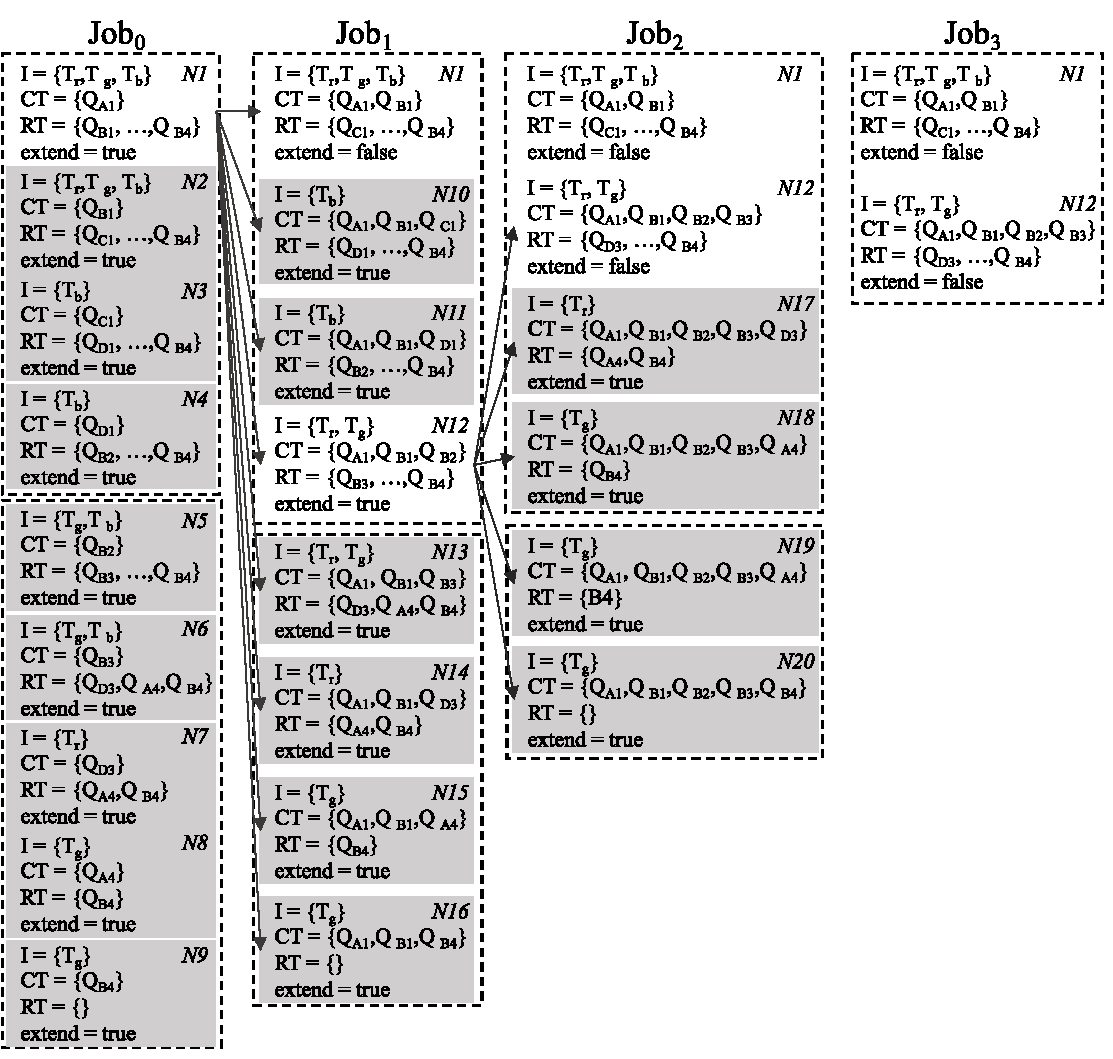
\includegraphics[scale=.5]{ctm.pdf}
% \caption{Enumeration tree for co-location patterns in \Cref{fig:patterns2} with $mCrd=2$ and $mSup=2$: each level of the enumeration tree corresponds to a distributed job.}
% \label{fig:ctminaction}
% \end{figure}
% \begin{example}[CTM in action]
% \Cref{fig:ctminaction} shows the enumeration tree for co-location patterns in \Cref{fig:patterns2} with $mCrd=2$ and $mSup=2$.
% Each level of the tree corresponds to an RDD generated in parallel through a job.
% RDDs are supposed to be composed by several partitions (dashed rectangles) distributed to executors.
% Each partition includes several nodes; the grayed ones are non-extendable.
% Examples of non-extendable nodes are $N2$ (redundant to $N1$) and $N3$ since $|N3.I| < mCrd$.
% The first level of the tree results from mapping of transactions to nodes carried out by \sf{MapQ()} (see \Cref{alg:colossal-distributed} Line \ref{alg:dist03}).
% Only the node $N1$ satisfies the $Check()$ for extensibility and is further expanded.
% Each of the following levels results from extending in parallel (see \Cref{alg:colossal-distributed} Line \ref{alg:dist15}) the nodes left over after pruning.
% Overall, two co-location patterns ($N1.I = \{T_b, T_g, T_r\}$ and $N12.I = \{T_g,T_r\}$) are found, marked with $extend=false$, retained in the RDD, and finally returned.
% \end{example}

% \section{Complexity analysis}\label{sec:complexity}
% CTM execution time is strictly related to the number of enumerated $\bar{\mathcal{Q}}$-itemsets. The worst-case in a row enumeration approach ($O(2^{|S|})$) takes place when all the trajectories move through all the tiles.
% The worst-case is not representative of the actual execution time, which varies enormously by changing the characteristics of the dataset (i.e., the number and shape of the trajectories) as well as the cardinality and support constraints.
% Here, we propose a probabilistic model to analyze how the number of \textit{Expected Itemsets} ($EI$) changes by varying such characteristics.

% We assume as given a tessellation of $|S|$ tiles (i.e., transactions), a dataset of trajectories $\mathcal{T}$ (i.e., items), the minimum group cardinality $mCrd$, and the minimum support $mSup$. Increasing the cardinality constraint $mCrd$ excludes the patterns involving a lower number of trajectories (see \Cref{alg:filterE} Line \ref{alg:filterE1}); similarly, increasing the support $mSup$ excludes the pattern generating from combinations of less than $mSup$ tiles (see \Cref{alg:filterE} Line \ref{alg:filterE2Val} and Line \ref{alg:filterE2Ext}).

% Henceforth, we assume that trajectories (i) have the same length $l$, (ii) are independent, and (iii) are uniformly distributed over the tiles.
% Then, the probability of a trajectory to go through exactly a set of tiles $\bar{S}$ such that $|\bar{S}|=\bar{s}$ is
% \begin{align}
% Pr(\bar{s}) = 
%     \begin{cases}
%     \frac{\binom{l}{\bar{s}}}{\binom{|S|}{\bar{s}}}, \bar{s} \le l \\
%     %\frac{l!/(l-\bar{s})!}{|S|!/(|S|-\bar{s})!}, l \le \bar{s} \\
%     0, otherwise
%     \end{cases}
% \end{align}
% \noindent where $\binom{l}{\bar{s}}$ computes the number of ways $\bar{s}$ tiles can be chosen out of a trajectory spanning $l$ tiles, while  $\binom{|S|}{\bar{s}}$ is the overall number of sets of $\bar{s}$ tiles out of the whole tessellation. 
% The probability to have at least $mCrd$ trajectories in $\bar{S}$ is
% \begin{align}
% Pr^+(\bar{s}) = 
%     \sum_{i=mCrd}^{|\mathcal{T}|} \binom{|\mathcal{T}|}{i}Pr(\bar{s})^i \cdot (1 - Pr(\bar{s}))^{|\mathcal{T}| - i}
% \end{align}
% where $Pr^+()$ is a Bernoulli trial \citep{papoulis1989probability} in which success/failure correspond to the presence/absence of a trajectory in the tile, and $\binom{|\mathcal{T}|}{i}$ is the number of sets of $i$ trajectories in $\mathcal{T}$.
% Finally, $EI$ is estimated by adding, for all the possible $\bar{S}$-itemset supports, the number of sets of tiles $\binom{|S|}{\bar{s}}$ times the probability each set of tiles has to contain at least $mCrd$ trajectories
% \begin{align}
% EI=\sum_{\bar{s}=1}^{|S|} \binom{|S|}{\bar{s}} \cdot Pr^+(\bar{s}) \le 2^{|S|}
% \end{align}
% Noticeably, the number of returned patterns (i.e., those spanning at least $mSup$ tiles) can be obtained by setting $\bar{s}=mSup$ in the summation above.

% \Cref{fig:complexity1} shows $EI$ by varying the dataset characteristics and the problem constraints.
% Solid lines represent trajectories with different lengths.
% To obtain a meaningful result, the length is expressed in relative terms with respect to the cardinality of the tessellation ($l/|S|=1$ if all the trajectories move through all tiles).
% The worst-case scenario (i.e., $EI=2^{|S|}$) takes place when $l/|S|=1$.
% Clearly, $EI$ increases for increasing values of $|S|$; however, the increase is limited for datasets with shorter trajectories.
% $EI$ further drops by constraining the patterns to include a greater amount of trajectories (\Cref{fig:complexity1}-right). 
% This proves that, despite the exponential complexity of the worst-case scenario, the expected complexity of CTM is orders of magnitude lower. 

% The model was applied to all datasets used to test CTM. While referring to \Cref{ssec:empcomp} for an in-depth analysis, we anticipate here that the model properly estimate $EI$ resulting in minimal deviations from the number of itemsets actually generated. 
% \begin{figure}[t]
% \centering
% 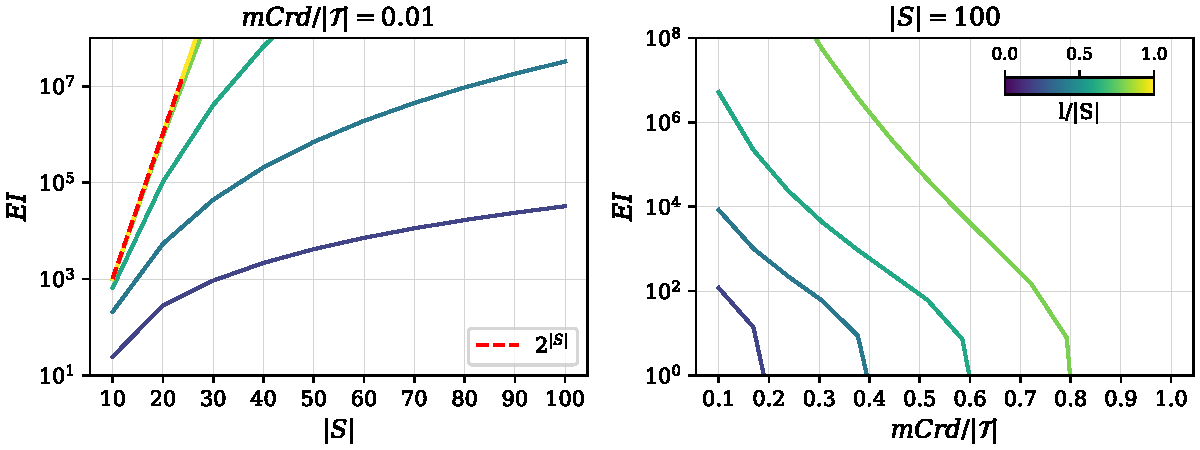
\includegraphics[scale=.42]{complexity3.pdf}
% \caption{Expected itemsets $EI$ varying (left) the number of tiles $|S|$ (with group-cardinality ratio $\frac{mCrd}{|\mathcal{T}|}=0.01$) and (right) the group-cardinality ratio (with $|S|=100$). Color codes the trajectory-length ratio $\frac{l}{|S|}$, trajectories move through all the tiles when $\frac{l}{|S|}=1$.}
% \label{fig:complexity1}    
% \end{figure}

% Table generated by Excel2LaTeX from sheet 'datasets'
% \begin{table}[t]
%   \scriptsize\centering
%   \caption{Dataset characteristics}
%   \label{tab:datasets}%
%     \begin{tabular}{l|ccc}
%     % \begin{tabular}{p{2cm}|p{1.6cm}p{1.8cm}p{1.8cm}}
%     \toprule
%      & \sf{Milan} & \sf{Oldenburg} & \sf{Hermoupolis}\\
%     \midrule
%     MOs & $6.0 \cdot 10^6$ & $10^6$ & $4.2 \cdot 10^3$ \\
%     Points & $2.2 \cdot 10^8$ & $6.4 \cdot 10^7$ & $5 \cdot 10^7$ \\
%     Avg traj. points & $23 \pm 97$ & $65 \pm 36$ & $1.2 \cdot 10^4 \pm 7 \cdot 10^3$ \\
%     Spatial span & $204 km^2$ & $634 km^2$ & $628 km^2$  \\
%     Time span & 3 months & 246 timestamps & 1 week \\
% %     \bottomrule
% %     \end{tabular}%
% % \end{table}%
% % % Table generated by Excel2LaTeX from sheet 'Sheet2'
% % \begin{table}[t]
% %     \centering
% %     \scriptsize\centering
% %     \caption{Features involved in pattern extraction.}
% %     \begin{tabular}{p{1.2cm}|p{1.6cm}p{1.2cm}p{1.8cm}}
%     % \toprule
%     % Features & \sf{Milan} & \sf{Oldenburg} & \sf{Hermoupolis} \\
%     \midrule
%     Dataset type & Real & Synthetic & Synthetic \\
%     Spatial feature & Administrative boundaries & Grid  & Grid \\
%     Temporal feature & Daily time slots & Minutes & Minutes \\
%     Additional features & - & - & Transportation, Activity, Speed \\
%     \bottomrule
%     \end{tabular}%
%     \label{tab:features}%
% \end{table}%

\section{Evaluation}\label{sec:test}
The approach has been implemented in Spark and is available at \url{https://github.com/big-unibo/ctm}.
All tests run on a cluster of 10 nodes, each equipped with an 8-core i7 CPU@3.60GHz and 16 GB of RAM and interconnected by Gigabit Ethernet.
We tested CTM on several use cases and scalability tests, but for the sake of space we only report the results on a real-world dataset.% \sf{Milan}.
% , \sf{Oldenburg}, and \sf{Hermoupolis}) we use to assess the \mf{
% \textit{effectiveness}, \textit{efficiency}, and \textit{robustness}
% } of our approach.
% As to effectiveness (\Cref{ssec:effec}), we (i) evaluate how CTM has been (or can be) applied to extract co-movement patterns in real-world (or synthetic) case studies including both geometric and semantic features, and (ii) assess the effects of semantic features on the co-movement patterns. %, and (iii) empirically evaluate the complexity model introduced in \Cref{sec:complexity}.
% As to efficiency (\Cref{ssec:efficiency}), we assess the scalability by changing the input parameters of CTM. 
% Finally, we compare CTM \mf{and its robustness} to related approaches in \Cref{ssec:comparison}.
% \subsection{Dataset description}
% The datasets differ with respect to MO behaviors and involved features.
% Their characteristics are summarized in \Cref{tab:datasets}.

\sf{Milan} is a real trajectory dataset that contains trajectories from $6 \cdot 10^6$ MOs (i.e., individuals) from the Milan metropolitan area (around $200 km^2$).
Trajectories are sparse in time since they represent inhabitants as well as travelers over three months.
% \sf{Milan} produces real-world patterns (e.g., from the main train station to well-known points of interest such as the dome or the stadium).
% \sf{Oldenburg} is a synthetic dataset \citep{DBLP:journals/geoinformatica/Brinkhoff02};
% %(see \cite{DBLP:journals/pvldb/HeCMPS15} for the generation process); 
% it contains trajectories from $10^6$ MOs from the Oldenburg area (around $600 km^2$).
% Since trajectories span for 246 timestamps, % and have an average length of 65 raw points.
% the synthetic trajectories are highly temporally overlapping and condensed in a small period of time.
% Hence, they are expected to produce co-movement patterns dense in space and time. % (e.g., assuming that a timestamp corresponds to a minute, trajectories span 4 hours at maximum).
% % \sf{Oldenburg} is a synthetic dataset and is not expected to produce realistic patterns
% \sf{Hermoupolis} is a synthetic dataset too \citep{DBLP:journals/sigspatial/PelekisSTT15}; its trajectories are annotated with additional features and come from $4.2 \cdot 10^3$ MOs from the Athens area (around $600 km^2$); trajectories span for 1 week and have an average length of $1.2 \cdot 10^4$ raw points.
% Additional features range from the means of transport (e.g., bus or bicycle) to the activity undertaken by the user (e.g., sporting, studying, relaxing), and to the speed (e.g., move or stop).
% % While \sf{Hermoupolis} is a synthetic dataset as well as \sf{Oldenburg}, trajectories are built to produce semantic realistic co-movement patterns (e.g., users moving in the same means of transport or doing the same activities).
% \subsection{Parameter tuning}
% $S$, $mCrd$, and $mSup$ are dataset- and problem-specific parameters (see \Cref{sec:related}) and have been chosen to answer the following business question: \textit{``Which computable patterns are meaningful for our analysis?''}.
% To do this we rely on the following guidelines.
% \begin{enumerate}
%     \item Choose a tessellation ($S$) according to the goal of the analysis (e.g., looking for co-movement patterns in the Milan neighborhoods).
%     If a geometric grid is adopted, the tile granularity depends on the level of detail of the analysis.
%     Note that the tessellation should depend on the goal rather than on the optimization of the computation time.
%     \item Set the number of shared tiles ($mSup$) that is relevant for the analysis (e.g., to be considered as interesting, a co-movement pattern must traverse at least 3 neighborhoods).
%     \item Set the minimum group cardinality ($mCrd$) that is relevant for the analysis (e.g., if interested in car-sharing applications $mCrd$ could be set between $2$ and $6$). 
%     \item Verify if the combination of parameters determines meaningful patterns in a reasonable amount of time.
%     If not, iterate on the parameters $mSup$ and $mCrd$ until (i) results are ``stable'' (i.e., varying $mCrd$ and $mSup$ causes limited changes in the number of co-movement patterns) as prescribed by the elbow method \citep{DBLP:conf/icdcsw/SatopaaAIR11}, and (ii) the solution is computable in a reasonable time.
%     While varying the parameters, consider the following.
%     \begin{itemize}
%         \item Higher values of $mCrd$ and $mSup$ entail a lower number of co-movement patterns (e.g., fewer groups of MOs will share a longer path) and, in turn, reduce the computation time. 
%         \item The values of $mCrd$ and $mSup$ should also consider the tessellation.
%         For instance, if trajectories are dense, a fine-grained tessellation determines longer patterns.
%         On the other hand, if trajectories are sparse, a fine-grained tessellation amplifies such sparsity reducing the MOs sharing the same tiles; thus, lower values of $mSup$ or $mCrd$ are needed to increase the number of returned patterns.
%     \end{itemize}
% \end{enumerate}
% Although automatizing the approach is beyond the scope of the paper, the points above encode the principles that should drive such an automatic solution.
%
% \subsection{Effectiveness}\label{ssec:effec}
% \subsubsection{Qualitative evaluation and setup of the tessellation}
%
\begin{table}[t]
\scriptsize\centering
\caption{KPIs by dataset and pattern type}
\label{tab:effpatterns}%
\begin{tabular}{l|ccccccc}
% \multicolumn{1}{c}{} & \multicolumn{7}{c}{\sf{Milan}} \\ % ($mCrd=100$, $mSup=12$) 
\toprule
Type    & $|S|$ & Patterns         & Enum.       & Time (s)  & Shape check & Card. check & Red. check \\
\midrule
Flow    & 88    & $9.7 \cdot 10^4$ & $2.1 \cdot 10^7$ & 31  & 53\%  & 82\% & 30\%\\
Co-locaction & 88    & $2.3 \cdot 10^5$ & $2.6 \cdot 10^7$ & 44  & 31\%  & 82\% & 31\%\\
Convoy\tablefootnote{Due to the sparsity in time, no convoy pattern is returned in the \sf{Milan} dataset. }  & 528   & 0                & $5.5 \cdot 10^8$ & 180 & 1\%   & 99\% & 90\%\\
Swarm   & 528   & $124$            & $3.0 \cdot 10^8$ & 127 & 8.2\% & 98\% & 70\%\\
\bottomrule
\end{tabular}%
% \\\vspace{10px}
% \begin{tabular}{l|cccc|cccc}
% \multicolumn{1}{c}{} & \multicolumn{4}{c}{\sf{Oldenburg} ($mCrd=500$, $mSup=12$)} & \multicolumn{4}{c}{\sf{Hermoupolis} ($mCrd=400$, $mSup=12$)} \\
% \toprule
% Type    & $|S|$    & Patterns & Enum. & Time (s)    & $|S|$          & Patterns         & Enum.       & Time (s)       \\
% \midrule
% Flow    & 90             & 12               & $4.6 \cdot 10^5$ & 11               & 230            & $9.3 \cdot 10^4$ & $2.2 \cdot 10^7$ & 34             \\
% Co-loc. & 90             & 42               & $4.6 \cdot 10^5$ & 14               & 230            & $9.3 \cdot 10^4$ & $2.4 \cdot 10^7$ & 36             \\
% Convoy  & $1.8\cdot10^3$ & $1.9 \cdot 10^4$ & $2.2 \cdot 10^9$ & $1.7 \cdot 10^3$ & $1.5\cdot10^3$ & $1.5 \cdot 10^5$ & $1.6 \cdot 10^9$ & 358            \\
% Swarm   & $1.8\cdot10^3$ & $6.5 \cdot 10^4$ & $2.4 \cdot 10^9$ & $1.8 \cdot 10^3$ & $1.5\cdot10^3$ & $1.0 \cdot 10^7$ & $2.7 \cdot 10^9$ & $1.1 \cdot 10^3$\\
% \bottomrule
% \end{tabular}%
\end{table}%
%
% \begin{figure}[t]
%     \centering
%     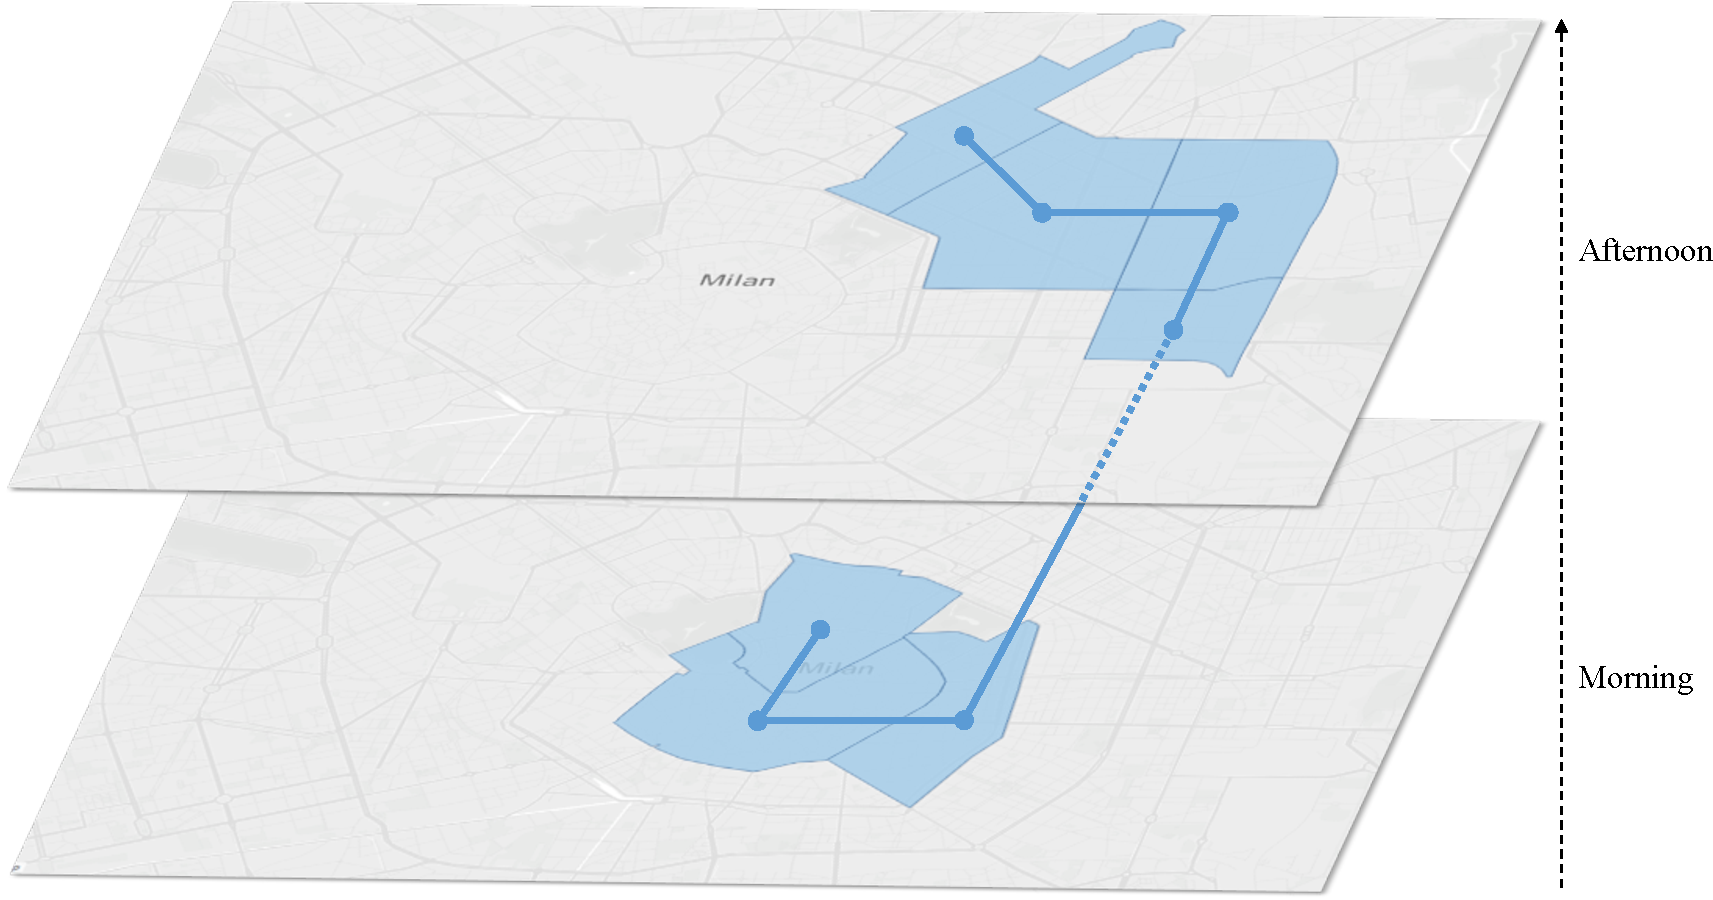
\includegraphics[scale=.3]{qualitativeswarm.pdf}
%     \caption{A real-world swarm pattern from the \sf{Milan} dataset with $mCrd=100$ and $mSup=7$.}
%     \label{fig:qualitativeswarm}
% \end{figure}
%
% To mine co-movement patterns with CTM, it is first necessary to identify the business question and then to properly set the tessellation. 
% Tessellations can be built out of diverse types of features, features can be continuous (e.g., speed) or discrete (e.g., means of transport), absolute (e.g., timestamp) or aggregated (e.g., hour bins), geometric (e.g., latitude/longitude) or semantic (e.g., administrative neighborhoods and municipalities, as in \Cref{fig:multilevtess}).
%
The dataset has been collected during the urban mobility analysis project \textit{``La città intorno''} (\url{https://lacittaintorno.fondazionecariplo.it/}) that aims to understand the mobility patterns of inhabitants living in suburban neighborhoods
% In the context of urban planning, \textit{``La città intorno''} focused 
and to rank neighborhoods by their attractiveness in order to understand how to allocate economic resources for requalification.
The attractiveness of a neighborhood is defined as the percentage of co-movement patterns passing through that neighborhood.
To fulfill the analysis, we initially define a tessellation where the spatial feature represents the 88 neighborhoods in Milan 
%(\Cref{fig:milnil}) 
and the temporal feature represents a relative dimension that partitions absolute timestamps into six bins, such as night (from 0 to 3) and morning (from 8 to 11); overall $|S| = 88 \cdot 6 = 528$ tiles.
Then, together with domain experts, we set relevant values for $mCrd$ (100) and $mSup$ (7). 
% \Cref{fig:qualitativeswarm} depicts an example of a swarm pattern for $mCrd=100$ and $mSup=7$ in which at least 100 people follow the same path around the city center in the morning and from the city center to the central station in the afternoon.
\Cref{tab:effpatterns} reports the outcomes for all co-movement pattern types.
\Cref{tbl:att} shows the results of our attractiveness analysis using swarm patterns, highlighting the need for higher requalification in ``Lodi - Corvetto", ``Padova", and ``Adriano"; the most attractive neighborhoods are the ones closest to the city center\footnote{By filtering tiles on the time bin, it is possible to characterize how attractiveness changes during the day.}.

\begin{table}[t]
    \centering
    \scriptsize
    \caption{An excerpt of attractiveness for neighborhoods in \sf{Milan}}
    \label{tbl:att}
    \begin{tabular}{lc}
    \toprule
        Neighborhood & Attractiveness \\
        \midrule
        Brera & 83\% \\ 
        Duomo & 83\% \\ 
        % Buenos Aires - Venezia & 82\% \\ 
        % XXII Marzo & 82\% \\
        % Gallaratese & 5\% \\ 
        Lodi - Corvetto & 4\% \\ 
        Padova & 3\% \\
        Adriano & 1\% \\ \bottomrule
    \end{tabular}
\end{table}

% We emphasize that while mapping raw trajectory points to tiles causes a loss of (geometric) precision, \textit{no semantic information is lost} as long as the chosen tessellation is adequate for the analysis goal.
% For instance, losing the precision of a single spatial point (in the order of meters) does not affect the results when looking for groups of trajectories moving through the neighborhoods.
% \Cref{tab:comp} shows compression obtained by mapping raw trajectory points into the tessellation to obtain the trajectory and the transaction datasets.
% Cardinality is expressed as raw points, tiles, and trajectory ids depending on CTM's step.

% \begin{table}[t]
% \centering
% \scriptsize
% \caption{Compression of the \sf{Milan} dataset}
% \label{tab:comp}
% \begin{tabular}{lccc}
% \toprule
% Dataset     & Raw              & Trajectory       & Transaction\\
% \midrule
% Cardinality & $2.2 \cdot 10^8$ & $2.9 \cdot 10^7$ & $3.8 \cdot 10^6$\\
% Size        & 6 GB              & 1.4 GB            & 19 MB            \\
% \bottomrule
% \end{tabular}
% \end{table}

% \begin{figure}[t]
%     \centering
%     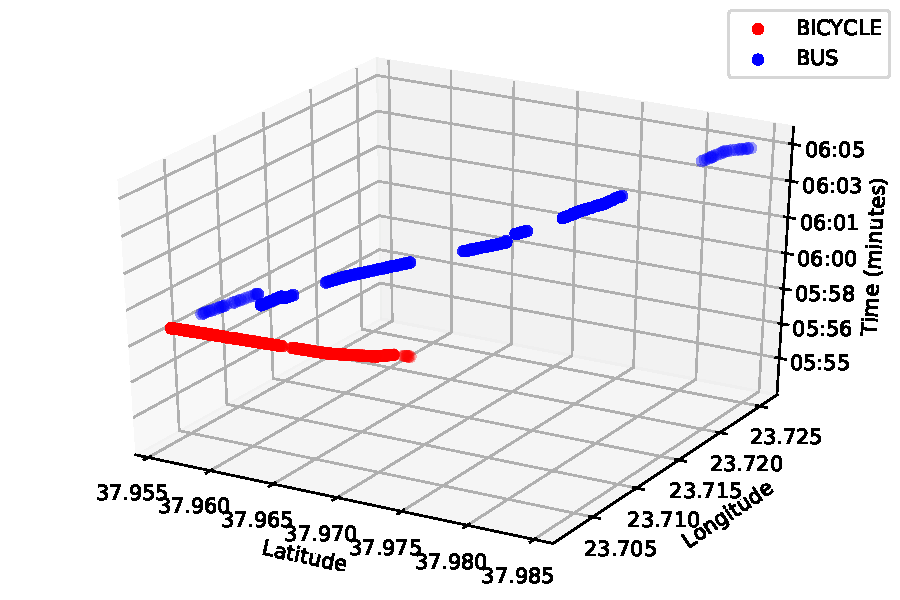
\includegraphics[scale=.55]{hermoupolis.pdf}
%     \caption{Example of a swarm pattern in the \sf{Hermoupolis} dataset including space, time, and means of transport (bus and bicycle) features.}
%     \label{fig:hermoupolis}
% \end{figure}

% \subsubsection{Impact of additional features}
% Since \sf{Oldenburg} and \sf{Hermoupolis} are synthetic datasets --- and no business value can be extracted from them --- we limit the spatial feature to a uniform grid and we shape the size of tiles to get a number of tiles that is comparable to \sf{Milan} (around 90), then we consider the time granularity of minutes for both of them.
% Additionally, \sf{Hermoupolis} contains the following features: means of transport, activity, and speed (i.e., move or stop).
% These features provide a more precise characterization of co-movement patterns.
% To highlight the effect of additional features (e.g., transport), \Cref{fig:hermoupolis} shows a qualitative example of a swarm composed of individuals moving together by bicycle and then by bus in the \sf{Hermoupolis} dataset.
% When moving by bus (blue), people share longer paths than by bicycle (red), and such paths are also more fragmented since no location can be registered in all adjacent tiles (due to the speed of the bus and the sampling rate of trajectory locations). 

% It is worth analyzing how much the patterns diverge when adding new features.
% We tested the \sf{Hermoupolis} dataset with and without its additional features ($mCrd=400$, $mSup=12$).
% We measured the differences in the co-movement pattern compositions through Adjusted Mutual Information (AMI) \citep{vinh2010information}.
% The higher (up to 1) the AMI, the higher the number of trajectories shared by co-movement patterns in the tessellations with and without additional features.
% If the AMI is 1, no information is induced by additional features.
% % no changes are induced by additional features in co-movement patterns (i.e., additional features do not bring additional information).
% \Cref{tab:ami} reports the results, where A, S, and T stand for additional, spatial, and temporal features.
% Additional features sensibly change co-movement patterns as desired.
% It should be also noted that the number of ST patterns can either increase or decrease with respect to STA patterns.
% This comes from the combined effect of two phenomena induced by the transition to a finer tessellation: on the one hand there is a proliferation of patterns, on the other hand, patterns could be sparser and, hence, filtered out.



% \begin{table}[t]
% \centering
% \scriptsize
% \caption{KPIs by pattern type}
% \label{tab:ami}%
% \begin{tabular}{lccc}
% \toprule
% Type    & AMI  & ST patterns & STA patterns\\
% \midrule
% Flow    & 0.17 & $5.1\cdot10^{3}$ & $9.3 \cdot 10^4$ \\
% Co-loc. & 0.17 & $5.6\cdot10^{3}$ & $9.3 \cdot 10^4$ \\
% Convoy  & 0.23 & $1.1\cdot10^{7}$ & $1.5 \cdot 10^5$ \\
% Swarm   & 0.23 & $1.1\cdot10^{7}$ & $1.0 \cdot 10^7$ \\
% \bottomrule
% \end{tabular}%
% \end{table}%

% \subsubsection{Complexity model evaluation}\label{ssec:empcomp}
% \Cref{fig:complexityemp} reports the empirical evaluation of the complexity model introduced in \Cref{sec:complexity}.
% We tested the model for co-location patterns on all our datasets to evaluate the gap between the estimated and actual number of generated itemsets (we recall that co-movement patterns are also itemsets).
% As to \sf{Hermoupolis}, we considered two tessellations including Spatio-Temporal features only (i.e., ST) or Spatio-Temporal with three additional features (i.e., STA).
% Noticeably the number of itemsets generated by CTM and $EI$ are in the same order of magnitude in all the cases but \sf{Hermoupolis} STA.
% This higher gap is due to the non-uniform distribution of the values of the additional features (e.g., there are more MOs moving than stopping, and more MOs moving by bus than by bicycle).
% % \eg{, which violates the uniformity assumption of the model}.
% However, even in this case, the gap between the empirical value and the theoretical one is by far smaller than the gap with the worst-case scenario, proving that our model provides an effective estimation.

% \begin{figure}[t]
%     \centering
%     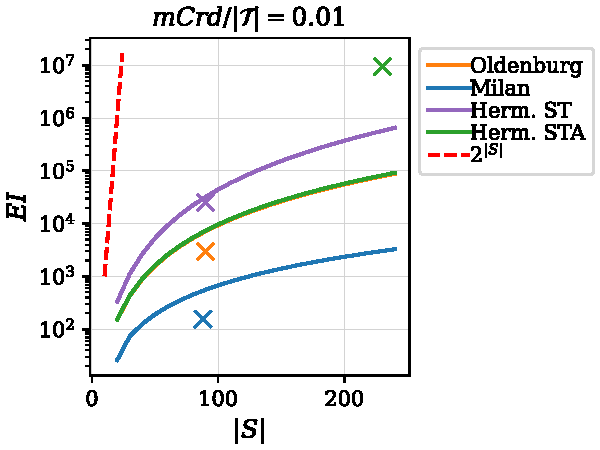
\includegraphics[scale=.65]{complexity-emp.pdf}
%     \caption{Worst-case (dashed line), theoretical (straight line), and empirical (mark) complexity for co-location patterns in \sf{Milan}, \sf{Oldenburg}, and \sf{Hermoupolis}. \sf{Oldenburg} and \sf{Hermoupolis} STA have overlapping theoretical complexities.}
%     \label{fig:complexityemp}
% \end{figure}

% \subsection{Efficiency}\label{ssec:efficiency}
% \begin{table}[t]
% \centering
% \scriptsize
% \caption{Parameters with default values}
% \label{tab:params}
% \begin{tabular}{clcc} % c
% \toprule
% Param.          & Description                   & \sf{Milan}        & \sf{Oldenburg}    \\%& \sf{Hermoupolis} \\
% \midrule
% $mCrd$          & Min. group cardinality        & 100               & 500               \\%& 500              \\
% $mSup$          & Min. shared path (support)    & 12                &  12               \\%&  12              \\
% $|S|$           & Tessellation cardinality      & 528               & $1.8 \cdot 10^3$  \\%& $1.5 \cdot 10^3$ \\ % Oldenburg 1791, Hermoupolis 1476
% $|\mathcal{T}|$ & Trajectories in the dataset   & $6.0 \cdot 10^6$  & $1.0 \cdot 10^6$  \\%& $4.2 \cdot 10^3$ \\
% Exec.           & Computational units           & 10                & 10                \\%& 10               \\
% RAM             & Available RAM per exec.       & 8 GB              & 8 GB                \\%& 8 GB               \\
% \bottomrule
% \end{tabular}
% \end{table}
% For the sake of conciseness, we focus on (i) the swarm pattern as it represents the scenario showing the highest computational time, and (ii)  \sf{Milan} and \sf{Oldenburg} datasets only since \sf{Hermoupolis} returns results highly similar to \sf{Oldenburg}.
% To study the performance in detail, we change the parameters in \Cref{tab:params}, one at a time, and we consider the respective default values for the remaining ones\footnote{As to RAM allocation, we assigned each executor 8 GB out of 16 GB since (i) a Spark-related memory overhead is assigned to each executor and (ii) the services responsible for cluster coordination have a non-negligible memory footprint.}.

% %The impact of the parameters discussed so far on the execution time is achieved by means of the pruning strategies presented in \Cref{sec:pruning}.
% The impact of pruning on the execution time is summarized in \Cref{tab:effpatterns}.
% % For the sake of brevity, we only report the results for \sf{Milan} since it is a real-world dataset. 
% For \sf{Milan}, the table shows the percentage of times each check has been triggered with respect to the enumerated $\bar{\mathcal{Q}}$-itemsets. While percentages are here reported independently of each other, a failure of one check prevents the computation of the others. In particular, the failure of the shape or cardinality checks allows to skip the support computation. 
% %With respect to the enumerated patterns, 
% The cardinality check is always the most effective pruning, preventing the extension of 98\% of $\bar{\mathcal{Q}}$-itemsets for swarm patterns.
% The shape check is more effective for flow patterns than for co-location patterns; extending $\bar{\mathcal{Q}}$-itemsets only within sets of connected tiles allows further pruning.

% \Cref{tab:effcard,tab:effsupp} show how performance changes by varying the minimum group cardinality (i.e., $mCrd$) and the minimum length of the shared path (i.e., the support $mSup$). 
% For all datasets the number of retrieved patterns and the computational time increase by decreasing the two thresholds.
% Decreasing $mCrd$ affects CTM more than decreasing $mSup$ due the higher pruning of the cardinality check.
% For instance, in \sf{Milan}, halving $mSup$ increases the enumerated nodes from $3.0 \cdot 10^{8}$ to $4.7 \cdot 10^{8}$, while halving $mCrd$ increases the enumerated nodes from $3.0 \cdot 10^{8}$ to $7.6 \cdot 10^{9}$. Indeed, cardinality checks sensibly affect the pruning (\Cref{tab:effpatterns}).

% \begin{table}[t]
% \scriptsize\centering
% \caption{Enumerated swarm patterns by increasing $mCrd$}
% \label{tab:effcard}%

% \begin{tabular}{ccc}
% \multicolumn{3}{c}{\sf{Milan}}\\
% \toprule
% $mCrd$ &         Enum. &          Time (s)     \\
% \midrule
%     25 &  $7.6\cdot10^{9}$ &  $1.5\cdot10^{3}$ \\
%     50 &  $1.5\cdot10^{9}$ &               398 \\
%     75 &  $5.8\cdot10^{8}$ &               186 \\
%    100 &  $3.0\cdot10^{8}$ &               126 \\
% \bottomrule
% \end{tabular}
% \begin{tabular}{ccc}
% \multicolumn{3}{c}{\sf{Oldenburg}}\\
% \toprule
% $mCrd$ &         Enum. &          Time (s) \\
% \midrule
% % 100 &  $4.5\cdot10^{10}$ &  $1.6\cdot10^{4}$ \\
% 200 &  $1.3\cdot10^{10}$ &  $6.0\cdot10^{3}$ \\
% 300 &   $6.6\cdot10^{9}$ &  $3.7\cdot10^{3}$ \\
% 400 &   $3.7\cdot10^{9}$ &  $2.6\cdot10^{3}$ \\
% 500 &   $2.4\cdot10^{9}$ &  $1.8\cdot10^{3}$ \\
% \bottomrule
% \end{tabular}
% 
% ~
% \begin{tabular}{ccc}
% \multicolumn{3}{c}{\sf{Hermoupolis}}\\
% \toprule
% $mCrd$ &              Enum. &          Time (s) \\
% \midrule
%   400 &   $2.7\cdot10^{9}$ &  $1.1\cdot10^{3}$ \\
%   425 &   $1.1\cdot10^{9}$ &               509 \\
%   450 &   $4.3\cdot10^{8}$ &               262 \\
%   475 &   $1.4\cdot10^{8}$ &               147 \\
%   500 &   $7.9\cdot10^{7}$ &               110 \\
% \bottomrule
% \end{tabular}
% \end{table}%

% \begin{table}[t]
% \scriptsize\centering
% \caption{Enumerated swarm patterns by increasing $mSup$}
% \label{tab:effsupp}%
% \begin{tabular}{ccc}
% \multicolumn{3}{c}{\sf{Milan}}\\
% \toprule
% $mSup$ &        Enum. & Time (s) \\
% \midrule
%      6 &  $4.7\cdot10^{8}$ &      349 \\
%      8 &  $3.2\cdot10^{8}$ &      180 \\
%     10 &  $3.2\cdot10^{8}$ &      148 \\
%     12 &  $3.0\cdot10^{8}$ &      126 \\
% \bottomrule
% \end{tabular}
% ~
% \begin{tabular}{ccc}
% \multicolumn{3}{c}{\sf{Oldenburg}}\\
% \toprule
% $mSup$ &  Enum. &         Time (s) \\
% \midrule
%  6 &  $2.7\cdot10^{9}$ &  $2.2\cdot10^{3}$ \\
%  8 &  $2.4\cdot10^{9}$ &  $1.8\cdot10^{3}$ \\
% 10 &  $2.4\cdot10^{9}$ &  $1.8\cdot10^{3}$ \\
% 12 &  $2.4\cdot10^{9}$ &  $1.8\cdot10^{3}$ \\
% \bottomrule
% \end{tabular}
% ~
% \begin{tabular}{ccc}
% \multicolumn{3}{c}{\sf{Hermoupolis}}\\\toprule
% $mSup$ &             Enum. & Time (s) \\
% \midrule
%      6 &  $1.2\cdot10^{8}$ &      132 \\
%      8 &  $1.2\cdot10^{8}$ &      151 \\
%     10 &  $7.9\cdot10^{7}$ &      126 \\
%     12 &  $7.9\cdot10^{7}$ &      110 \\
% \bottomrule
% \end{tabular}

% \end{table}%

% \Cref{tab:efftiles,tab:efftraj} show how performance changes by varying the cardinality of both the tessellation (i.e., $|S|$) and the trajectories (i.e., $|\mathcal{T}|$) given as input to CTM.
% As to $|S|$, we achieve finer tessellations by creating finer spatial grids. To do so in the \sf{Milan} dataset, we approximate the neighborhoods with a spatial grid.
% For all datasets, we start with a grid of cells with side $2km$ and we incrementally reduce the cell side by 200 meters.
% Changing the tessellation cardinality $|S|$ affects CTM in two ways.
% On the one hand, increasing the cardinality affects the sparsity of the dataset.
% Having more tiles fragments trajectory groups until only trajectories matching \textit{exact} points (e.g., latitude and longitude) can be grouped.
% On the other hand, it broadens the search space of the algorithm.
% % Interestingly 
% These two effects compensate each other, allowing CTM to explore a search space in the order of thousands of tiles.
% As to $|\mathcal{T}|$, we achieve smaller datasets by halving the number of trajectories twice;
% decreasing the trajectory cardinality $|\mathcal{T}|$ sensibly reduces the enumerated space and the computational time:
% %  Intuitively, as shown in 
% fewer trajectories are less likely to create 
% %groups with a sufficient cardinality and support 
% co-movement patterns. % (see \Cref{sec:complexity}).

% \begin{table}[t]
% \scriptsize\centering
% \caption{Performance for increasing tiles $|S|$}
% \label{tab:efftiles}%

% \begin{tabular}{ccc}
% \multicolumn{3}{c}{\sf{Milan}}\\
% \toprule
% $|S|$ &        Enum. & Time (s) \\
% \midrule
% 357 &  $3.0\cdot10^{8}$ &      126 \\
% 534 &  $9.6\cdot10^{8}$ &      288 \\
% 679 &  $1.4\cdot10^{9}$ &      399 \\
% 873 &  $2.0\cdot10^{9}$ &      647 \\
% \bottomrule
% \end{tabular}
% ~
% \begin{tabular}{ccc}
% \multicolumn{3}{c}{\sf{Oldenburg}}\\
% \toprule
% $|S|$ &          Enum. &          Time (s) \\
% \midrule
% 1791 &  $2.4\cdot10^{9}$ &  $1.8\cdot10^{3}$ \\
% 1838 &  $2.5\cdot10^{9}$ &  $1.9\cdot10^{3}$ \\
% 2101 &  $2.2\cdot10^{9}$ &  $1.6\cdot10^{3}$ \\
% 2232 &  $2.8\cdot10^{9}$ &  $2.0\cdot10^{3}$ \\
% \bottomrule
% \end{tabular}
% ~
% \begin{tabular}{ccc}
% \multicolumn{3}{c}{\sf{Hermoupolis}}\\\toprule
% $|S|$ &             Enum. &          Time (s) \\
% \midrule
%   141 &  $2.6\cdot10^{9}$ &  $3.7\cdot10^{3}$ \\
%   150 &  $7.9\cdot10^{7}$ &               110 \\
%   158 &  $6.7\cdot10^{9}$ &  $4.2\cdot10^{3}$ \\
%   160 &  $4.4\cdot10^{7}$ &                71 \\
%   179 &  $8.4\cdot10^{8}$ &               415 \\
% \bottomrule
% \end{tabular}
% \end{table}%

% \begin{table}[t]
% \scriptsize\centering
% \centering
% \caption{Performance for increasing trajectories $|\mathcal{T}|$}
% \label{tab:efftraj}%
% \begin{tabular}{p{0.9cm}p{0.9cm}p{1.0cm}}
% \multicolumn{3}{c}{\sf{Milan}}\\
% \toprule
%   $|\mathcal{T}|$ &        Enum. & Time(s) \\
% \midrule
%  $1.5\cdot10^{6}$ &  $1.6\cdot10^{7}$ &       10 \\
%  $3.0\cdot10^{6}$ &  $6.2\cdot10^{7}$ &       22 \\
%  $6.0\cdot10^{6}$ &  $3.0\cdot10^{8}$ &      126 \\
% \bottomrule
% \end{tabular}
% \begin{tabular}{p{0.9cm}p{0.9cm}p{1.0cm}}
% \multicolumn{3}{c}{\sf{Oldenburg}}\\
% \toprule
%   $|\mathcal{T}|$ &        Enum. &          Time(s) \\
% \midrule
%  $2.5\cdot10^{5}$ &  $5.7\cdot10^{7}$ &                43 \\
%  $5.0\cdot10^{5}$ &  $4.1\cdot10^{8}$ &               273 \\
%  $1.0\cdot10^{6}$ &  $2.4\cdot10^{9}$ &  $1.8\cdot10^{3}$ \\
% \bottomrule
% \end{tabular}
% ~
% \begin{tabular}{ccc}
% \multicolumn{3}{c}{\sf{Hermoupolis}}\\\toprule
%   $|\mathcal{T}|$ &             Enum. & Time (s) \\
% \midrule
%  $1.0\cdot10^{3}$ &  $1.3\cdot10^{5}$ &       13 \\
%  $2.0\cdot10^{3}$ &  $5.6\cdot10^{6}$ &       19 \\
%  $4.2\cdot10^{3}$ &  $7.9\cdot10^{7}$ &      109 \\
% \bottomrule
% \end{tabular}
% \end{table}%

% Finally, \Cref{tab:efframexec} shows how the amount of RAM and parallelism (i.e., the number of executors) affect CTM.
% As shown for all datasets, our approach can be applied even when a small amount of RAM is given to each executor.
% This is due to our implementation on Spark RDDs, where data is split into partitions that are loaded into main memory only when they are ready to be processed.
%This is due to our Spark implementation.
%An RDD collects a huge amount of data that cannot fit into a single machine.
%Spark partitions RDDs and distributes the partitions across different nodes.
%A partition is an atomic chunk of data stored on a node in the cluster.
%Partitions are basic units of parallelism that are loaded into main memory only when they are ready to be processed.
% As to the parallelism, reducing the number of executors sensibly affects performance.
% When CTM runs on a single executor, we move from 2 to 13 minutes in \sf{Milan} and from 30 minutes to almost 4 hours in \sf{Oldenburg}.
% %while the RAM per executor is not critical for the execution time, 
% The number of executors affects time (almost) linearly, proving that CTM uniformly distributes the workload among the executors.
% Note that changing RAM and number of executors does not affect the result in terms of the generated co-movement patterns but only the time necessary for their extraction.

% \begin{table}[t]
% \scriptsize\centering
% \caption{Time (sec.) for increasing RAM and executors}
% \label{tab:efframexec}%

% \begin{tabular}{ccc}
% \toprule
% RAM &  \sf{Milan} &  \sf{Oldenburg} \\%& \sf{Hermoupolis} \\
% \midrule
% 2 GB & 131 & $1.8\cdot10^{3}$ \\%& 104\\
% 4 GB & 122 & $1.9\cdot10^{3}$ \\%& 109\\
% 6 GB & 122 & $1.7\cdot10^{3}$ \\%& 106\\
% 8 GB & 126 & $1.8\cdot10^{3}$ \\%& 110\\
% \bottomrule
% \end{tabular}
% ~
% \begin{tabular}{ccc}
% \toprule
% Executors & \sf{Milan} & \sf{Oldenburg} \\%& \sf{Hermoupolis}\\
% \midrule
% 1  & 849 & $1.3\cdot10^{4}$ \\%& 635\\
% 3  & 297 & $4.6\cdot10^{3}$ \\%& 232\\
% 6  & 172 & $2.6\cdot10^{3}$ \\%& 146\\
% 10 & 126 & $1.8\cdot10^{3}$ \\%& 110\\
% \bottomrule
% \end{tabular}
% \end{table}%
 
% We proved that CTM can work in the order of thousands of tiles (\Cref{tab:effpatterns}).
% However, it is unfeasible to provide fixed boundaries in which the method can be applied since they depend on the following factors.
% \begin{itemize}
%     \item The distribution of trajectories. Intuitively, $10^4$ tiles with highly sparse trajectories can produce fewer co-movement patterns than $10^2$ tiles with dense trajectories. %, see our complexity model in \Cref{fig:complexity1}.
%     \item The pruning effects of $mSup$ and $mCrd$ (\Cref{tab:effpatterns}). Even out of a huge number of tiles, the higher is $mCrd$ the easier it becomes to discard \textit{a-priori} tiles with insufficient amounts or trajectories.
%     \item The combination of the above: given a certain dataset, choosing finer tessellations (i.e., tessellations with an increasing number of tiles) affects the cardinality and support of the extracted co-movement patterns (e.g., smaller tiles will contain fewer trajectories requiring a different value of $mCrd$ to extract meaningful co-movement patterns).
% \end{itemize}

% \subsection{Comparison}\label{ssec:comparison}
% \mf{
Finally, we tested CTM against SPARE \citep{DBLP:journals/pvldb/FanZWT16} (the only big-data approach to the extraction of \textit{generic} co-movement patterns), and PFPGrowth \citep{DBLP:conf/recsys/LiWZZC08} (a big data approach to Frequent Itemset Mining) on two synthetic datasets \sf{Oldenburg} and \sf{Hermoupolis}.
For the sake of space, the details of the scalability testing process are omitted and are available in the extended version \cite{DBLP:journals/eswa/FranciaGG24}.
Overall, CTM scalability proves to be better than the others for big groups of trajectories.

% Before diving into the comparison, we first list the main features distinguishing CTM and SPARE.
% }
% \begin{itemize}
% \item CTM allows the extraction of spatial patterns %(flow and co-location; where flow also requires checking whether trajectories move through adjacent tiles) 
% as well as patterns characterized by custom features (e.g., time, speed, or age) of which a discussion has been presented at the end of \Cref{sec:modeling}.
% SPARE extracts \textit{only} spatio-temporal patterns and does not provide support to additional features.
% \item The temporal feature is optional in CTM and can have \textit{custom} semantics, allowing, for instance, the extraction of co-movement patterns in weeks, holidays, or absolute hour bins. SPARE requires a mandatory \textit{absolute} temporal feature. 
% \item SPARE treats the temporal and spatial features sequentially. At first, it groups trajectory points by absolute time bins (e.g., 3 Mar 2020, 10:00:00 and 3 Mar 2020, 11:00:00), then it clusters trajectories in each time bin, and, finally, it uses an Apriori-like approach to create the co-movement patterns out of the clusters from different time bins.
% This results in the lack of possibility to find co-movement patterns within the same time bin.
% As a result, if the time bin is coarse (e.g., morning or afternoon) a sensible amount of co-movement patterns is lost (e.g., individuals that move from one side of Milan to the other in a hour).
% \item Due to their formulation, CTM and SPARE are complementary.
% CTM allows the retrieval of large groups of trajectories from a coarse tessellation (which justifies the adoption of a bread-first row-enumeration approach), while SPARE allows the retrieval of smaller groups from a finer path (which justifies the adoption of an Apriori-like enumeration).
% As a result, when SPARE tries to extract huge groups of trajectories, it easily ends up in a memory fault.
% \end{itemize}


% \mf{
% While SPARE does not consider additional features, Frequent Itemset Mining approaches could be leveraged to compute \textit{all} FIs and then filter out only the actual co-movement patterns through a post-processing phase\footnote{Note that any algorithm for FIM can be picked}.
% We leverage PFPGrowth, a well-known implementation of distributed FIM already implemented in the Spark suite, to compute \textit{all} the (potential) swarm patterns on the entire \sf{Oldenburg} dataset.
% In PFPGrowth the computation of FIs does not rely on Apriori enumeration. 

% We tested SPARE against the whole $\sf{Oldeburg}$, $\sf{Hermoupolis}$, and $\sf{Milan}$ datasets and we stopped computations longer than $10^4$ seconds.
% SPARE failed to compute due to the exponentiality of Apriori enumeration.
% }
% The points above explain why, by construction, it is unfeasible to have exactly the same co-movement patterns unless the time bin is fine-grained enough to guarantee that no trajectory has more than one location in the same bin. With this in mind, we tried to make the comparison as fair as possible by:
% % \begin{itemize}
% %     \item Narrowing the comparison down to \sf{Oldenburg} by only varying the minimum support since SPARE is limited to an absolute time dimension and cannot handle additional semantic features (\sf{Milan} was too sparse to produce meaningful results).
% %     \item Reducing the time bin granularity in the order of seconds so that no trajectory has more than one location in the same time bin. This increased the size of the tessellation to $|S|=3422$.
% %     \item Reducing $mCrd$ to 10 and sampling trajectories down to $|T|=2000$. This is necessary since SPARE follows an Apriori enumeration that is exponential in the number of trajectories in the co-movement patterns.
% % \end{itemize}
% \mf{
% \begin{itemize}
%     \item \sf{Oldenburg}: the time bin granularity is set in the order of seconds so that no trajectory has more than one location in the same time bin; this increased the size of the tessellation to $|S|=3422$. We sampled only 2000 trajectories out of $10^6$ (i.e., $|T|=2000$); this is necessary since SPARE follows an Apriori enumeration that is exponential in the number of trajectories in the co-movement patterns.
%     \item \sf{Hermoupolis}: we dropped the additional semantic features since SPARE is limited to an absolute time dimension and we sampled only 200 trajectories out of $4.2 \cdot 10^3$ (i.e., $|T|=200$).
%     \item \sf{Milan} is too sparse in time to produce meaningful results at a fine time-space granularity and with a limited amount of trajectories.
% \end{itemize}
% }

\begin{figure}[t]
    \centering
    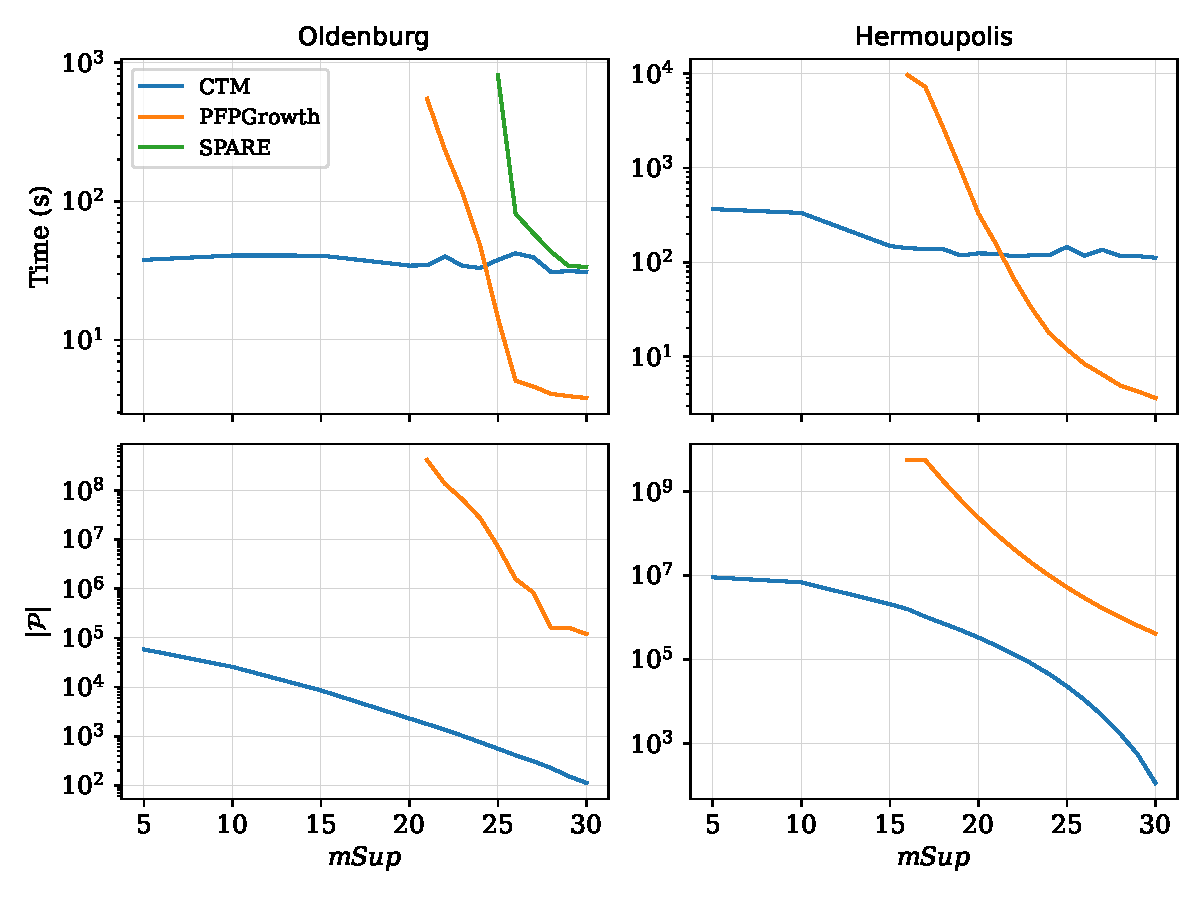
\includegraphics[scale=.45]{comparison_mSup.pdf}
    \caption{\mf{Comparing CTM, SPARE, and PFPGrowth in terms of computational time (top) and co-movement patterns (bottom).}}
    \label{fig:comparison}
\end{figure}

% \mf{
% \Cref{fig:comparison} depicts the comparison of the three approaches in terms of computational times and number of retrieved patterns (with the same hardware and software configurations).

% \begin{itemize}
%     \item CTM and SPARE retrieve the same patterns (i.e., their $|P|$ lines are overlapping).
%     However, following an Apriori-like strategy, SPARE performance highly depends on the minimum support: the lower it is, the higher the likelihood of extracting patterns with sufficient cardinality and the wider the portion of search space to be enumerated.
%     This results in memory faults when $mSup$ is below 25 even in the modified $\sf{Oldenburg}$ dataset and the computation is stopped after three hours in the modified $\sf{Hermoupolis}$ dataset already for $mSup=30$ (there is no green line in the top-right chart). 
%     Conversely, in CTM the computational time is less affected by the minimum support. %but rather depends on the cardinality of the tessellation. 
%     \item As to PFPGrowth, although both FIs and co-movement patterns decrease by increasing the $mSup$ threshold (as expected, the higher $mSup$ the lower the valid patterns), the number of FIs to post-process remains orders of magnitude higher than the co-movement patterns, and with lower supports their extraction becomes orders of magnitude slower \citep{DBLP:journals/tkde/LuccheseOP06}.
%     This makes FIM approaches strongly inefficient.
% \end{itemize}
% We close this section with a remark on the robustness of the algorithm. The tests shown above for CTM on different datasets and its comparison against different algorithms show that its performance is stable and is not the result of overfitting to a specific dataset or configuration.
% }
% %Finally, we emphasize that even restricting the trajectory dataset to $|\mathcal{T}|=2000$ makes SPARE fail due to the exponentiality determined by the Apriori-like strategy.

\section{Conclusion}\label{sec:conclusion}
CTM is a big-data approach to extract spatial and spatio-temporal mobility patterns possibly enriched by additional trajectory features that characterize behavioral mobility patterns.
With respect to the existing literature, CTM is general-purpose as it provides a unifying approach to extract different pattern types and is particularly suited for applications characterized by a high number of trajectories to be analyzed on a feature space with limited cardinality (e.g., to capture 
%the human behaviors, such as 
the daily commuting of a citizen through different neighborhoods, rather than analyzing her detailed path at the single street level).
% Tests show that in this context CTM is by far more efficient and expressive than previous general-purpose approaches.
As new research directions, we plan to: (i) introduce a definition of \textit{group cohesion} to further prune mobility patterns based on the shared tiles, (ii) investigate how the extracted mobility patterns can be summarized in a more succinct representation, (iii) investigate how gridding affects the stability of co-movement patterns, and (iv) consider a unifying extraction of mobility patterns from streaming trajectory data in order to apply CTM to online location-based systems.

% \appendix

% \section{Proofs of theorems}\label{ap:proof}

% \begin{proof}[Closeness of $\bar{\mathcal{Q}}$-itemset]\label{ap:t1}
% We show by contradiction that (i) all $\bar{\mathcal{Q}}$-itemsets are closed, and (ii) all closed itemsets are $\bar{\mathcal{Q}}$-itemsets.
% As to (i), if a $\bar{\mathcal{Q}}$-itemset $I$ is not closed, by definition there exists an itemset $I' \supset I$ such that $\sup(I')=sup(I)$; in this case, items in $I' \setminus I$ would be shared by all transactions in $\bar{\mathcal{Q}}$, contradicting the definition of $\bar{\mathcal{Q}}$-itemset.
% As to (ii), if a closed itemset $I$ is not a $\bar{\mathcal{Q}}$-itemset, there exists an item $t \not \in I$ shared by all transactions in $\bar{\mathcal{Q}}$, but in this case $sup(I \cup \{t\})=sup(I)$, contradicting the closeness definition.
% \end{proof}

% \begin{proof}[Uniqueness of non-redundant enumeration nodes]\label{ap:t2}
% The proof follows two statements: (i) lexicographic ordering in CTM guarantees that enumeration sequences are unique, thus  $N.CT \neq N'.CT$ even if $N.I=N'.I$, and (ii) every $\bar{\mathcal{Q}}$-itemset $I$ is generated by intersecting transactions belonging to its support, which is $N.CT \subseteq sup(I)$.
% From (i) and (ii) follows that there exists only one enumeration such that $N.CT = sup(I)$.
% \end{proof}

% \begin{proof}[Completeness of non-redundant enumerations]\label{ap:t3}
% If $N'$ is redundant there must exist a non-redundant node $N$, such that $N.I=N'.I$ and  $N.CT \supset N'.CT$.
% More precisely, according to \Cref{alg:colossal} Line \ref{alg:col04}, transactions in $N.CT$ that are not in $N'.CT$ must have lower ids than those in $N'.CT$.
% Formally, $N.CT = N'.CT \cup \mathcal{Q}^*$ where, $ \forall (Q^*,Q')$ with $Q^* \in \mathcal{Q}^* \subseteq \mathcal{Q}$ and $Q' \in N'.CT$, it is $id(Q^*)<id(Q')$.
% According to the CTM enumeration strategy $N.RT \supseteq N'.RT$.
% Thus, every extension obtained from $N'$ will be obtained extending $N$ too.
% \end{proof}

\balance
\bibliography{refs}

\end{document}